\documentclass[10pt]{article}
\input preamble.tex

\title{Final Report}
\author{Arnika Chidambaram \and Caroline Hughes \and Mitch Negus}

\bibliography{ne255-sources}

\begin{document}
\maketitle

\tableofcontents

%%%%%%%%%%%%%%%%%%%%%%%%%%%%%%%%%%%%%%%%%%%%%%%%%%%%%%%%%%%%%%%%%%%%%%%%
%%  INTRODUCTION -- What does the code we wrote do/what is the problem
%%      we solved? High level motivation/purpose? Preview what we are
%%      going to talk about.
%%%%%%%%%%%%%%%%%%%%%%%%%%%%%%%%%%%%%%%%%%%%%%%%%%%%%%%%%%%%%%%%%%%%%%%%
\newpage
\section{Introduction}
\label{sec:intro}
%\sectionauthor{Arnika}

The purpose of this project is to study variance reduction methods in Monte Carlo using deterministic methods.The goal is to create an importance map for the Monte Carlo game and selecting parameters is an important step in deterministic calculations. 
After parameters are selected, a map that accelerates the Monte Carlo calculation while simultaneously lowering deterministic cost, is created. Deterministic methods provide fast solutions to the transport equation, and require relatively simple inputs. Currently there is high demand for a reliable and efficient transport methods that can be used to solve complex fixed source problems\cite{slaybaugh:deterministic-parameter-study}.


Two variance reduction methods that use deterministic methods are Consistent Adjoint Driven Importance Sampling (CADIS) and Forward Weighted-Consistent Adjoint Driven Importance Sampling (FW-CADIS). CADIS optimizes specific, local response functions, where as FW-CADIS optimizes global response functions of this work. 

Throughout the course of this report, the mathematics behind variance reduction and the adjoint problem will be explained. After that, an overview of CADIS AND FW-CADIS will be given, and then the algorithms for ADVANTG and MCNP inputs and outputs will be provided. Finally, seven test cases will be run using CADIS and FW-CADIS and results will be plotted in VisIt. 


%%%%%%%%%%%%%%%%%%%%%%%%%%%%%%%%%%%%%%%%%%%%%%%%%%%%%%%%%%%%%%%%%%%%%%%%
%%  MATHEMATICS -- Write the continuous and discretized equations we are
%%      solving and define all terms. Include overview of derivations.
%%%%%%%%%%%%%%%%%%%%%%%%%%%%%%%%%%%%%%%%%%%%%%%%%%%%%%%%%%%%%%%%%%%%%%%%
\section{Mathematics}
\label{sec:math}

%%%%%%%%%%%%%%%%%%%%%%%%%%%%%%%%%%%%%%%%%%%%%%%%%%%%%%%%%%%%
%%  VARIANCE REDUCTION
%%%%%%%%%%%%%%%%%%%%%%%%%%%%%%%%%%%%%%%%%%%%%%%%%%%%%%%%%%%%
\subsection{Variance Reduction} % Mitch
\label{sec:math:var-red}
%\sectionauthor{Mitch}

Monte Carlo simulations have the unique advantage of being continuous and entirely free from the effects of discretization choices that are present in deterministic simulations; however, they tend to be much more computationally expensive.
In analog Monte Carlo simulations, enormous numbers of particle histories must often be tracked to produce ample statistics for meaningful results.

To meet these criteria and be considered meaningful, data must sufficiently cover the solution space and have a low statistical uncertainty, represented by a small variance.
The variance (the square of the standard deviation, $\sigma$) is defined as the squared sum of the deviation of each datapoint from the mean, $\bar{x}$, divided by the number of degrees of freedom in the problem (one less than the totlal number of datapoints) \cite{hughes}:

\begin{equation*}
\sigma^{2} = \frac{\sum_{i}^{N}{\left(x_{i}-\bar{x}\right)^{2}}}{N-1} ,
\end{equation*}
%
where $N$ is the number of particle histories included in the calculation.
Since the particle histories (and therefore $x_{i}$) are independent, the central limit theorem applies.
It follows that the standard deviation of the mean, $S_{\bar{x}}$, decreases proportionally to $1/\sqrt{N}$.
For comparative purposes, this measure is usually represented by the relative error, $R$, where

\begin{equation*}
R \equiv \frac{S_{\bar{x}}}{\bar{x}} = \frac{\sigma^{2}}{\bar{x}\sqrt{N}}.
\end{equation*}
%
More particles lead directly to a reduced uncertainty.

While simulating more particles is beneficial for reducing uncertainty in a simulation, it unsurprisingly increases the time needed for simulation.
In general, the efficiency of a simulation is given by its figure of merit (FOM), defined as

\begin{equation*}
\text{FOM} \equiv \frac{1}{R^{2}T}.
\end{equation*}
%
$R$ is the relative error and $T$ is the computer time taken for the simulation \cite{software:mcnp5}.
Assuming independent particles, the run time $T$ is directly proportional to the number of particles: $ T \propto N $.
When the dependencies of both $R$ and $T$ on $N$ are considered, the FOM becomes constant and no substantial gains are made in terms of performance for more particles ($\;R^{2}T \propto (1/\sqrt{N})^{2}N = const.\;$ ).

Specific variance reduction methods attempt to circumvent this dilemma using a variety of clever techniques.
Often, these methods emphasize simulations in regions of the problem space that have the strongest contributions to the final solution, gleaning deeper insights without wasting as much computation as analog Monte Carlo simulations.
Examples include truncation methods, population control methods, modified sampling methods, and partially-deterministic methods. For maximal effect, several of these methods may be employed together in a given simulation. Some of these methods are described below.

Truncation methods are undoubtedly the most common variance reduction technique, whereby the problem space is restricted in some dimension (technically, truncation methods are employed in almost every Monte Carlo simulation to some degree, as finite boundaries must exist on space, particle energy, time, etc.).
Truncation methods speed up calculations by avoiding simulation of parts of a problem that will not contribute to the solution.
While easy to incorporate into a simulation, care must be taken to ensure that these parts of the problem space actually \textit{will not}, as opposed to just \textit{should not}, contribute to the solution.

Population control methods allow more flexibility in sampling areas of importance in the phase space, and can be separated into two categories: splitting and rouletting.
In both cases, particles are assigned weights that are adjusted depending on the particle's importance to the final solution.
Splitting takes place when a particle enters an area of higher importance, since it is most important that the variance be low in this region.
By dividing the particle into multiple copies, the total number of particle histories in the simulation, $N$, can be artificially inflated, and the relative error reduced.
In order to preserve the initial particle's weight, $w$, on the final solution, the new $n$ split copies are scaled appropriately by a factor of $w$/$n$.

\begin{equation*}
\sum_{i}^{n}{\frac{w}{n}} = n\left(\frac{w}{n}\right) = w
\end{equation*}
%
Conversely, if a particle travels into a region of lower importance, the particle will undergo a ``game'' of Russian roulette, with a survival probability of $1/n$.
In this way, we reduce the number of particles that must be tracked, thereby reducing the time $T$ of the simulation.
The relative error of the desired solution will experience less impact since these rouletted particles are in areas of low importance and less likely to contribute to that solution.
Any particle that survives will have it's initial weight, $w$, increased by a factor of $n$, so that on average the total weights are conserved.

In addition to the splitting and rouletting routines, weight window restrictions are often placed on the simulation so that weights do not become too large or too small.
Particles with large weights will be split to prevent any one particle from having too much effect on the final solution, while particles with small weights will be rouletted to prevent the simulation from wasting time tracking essentially meaningless histories.

Population control methods influence the number of particles based on where they travel, weighting them accordingly.
Similarly, modified sampling methods use adjusted probability distributions to control the number of particles generated with a given set of initial conditions and weight those particles accordingly.
If a given situation ought to occur with probability $P$, a modified sample would generate that same situation with probability $P'$, but with weight $w_{\text{new}} = P/P'$.
The overall probability is preserved:
\begin{equation}
P = w_{new} \cdot P' = \frac{P}{P'}P'
\label{eq:prob-preserved}
\end{equation}
but the number of particles is adjusted to more effectively contribute to the solution and reduce the variance.



%%%%%%%%%%%%%%%%%%%%%%%%%%%%%%%%%%%%%%%%%%%%%%%%%%%%%%%%%%%%
%%  The Adjoint Problem
%%%%%%%%%%%%%%%%%%%%%%%%%%%%%%%%%%%%%%%%%%%%%%%%%%%%%%%%%%%%
\subsection{The Adjoint Problem}
\label{sec:math:adjoint}

In general, the adjoint $A^\dagger$ of an operator, function, or matrix $A$ is the complex conjugate of the transpose of $A$ \cite{boas}.
It has the property:

%%%%%%%%%%%%%%%%%%%%%%%%%%%%%%%%%%%%%%%%%%%%%%%%
\begin{equation}
\left< \psi^\dagger, A \psi \right> =
\left< \psi A^\dagger, \psi^\dagger \right>
,
\label{eq:adjoint-property}
\end{equation}
%%%%%%%%%%%%%%%%%%%%%%%%%%%%%%%%%%%%%%%%%%%%%%%%
where $\left< \;\cdot\; \right>$ represents ``integration over all independent variables,'' which, in phase space, is given by \cite{lewis-and-miller}

\begin{equation*}
\left< \;\cdot\; \right> = \int d^3\vec{r} \int dE \int d\hat{\Omega}
\end{equation*}
%
The adjoint of the Boltzmann Neutron Transport equation (TE) represents the importance of the contribution of a particle at a particular location, time, energy, and angle to an objective function such as detector source \cite{wagner:automated-variance-reduction}.
For the transport operator, $H$, defined in \cref{eq:transport-operator}, the adjoint transport operator $H^\dagger$ can be derived using the property given in \cref{eq:adjoint-property} and is defined in \cref{eq:adjoint-transport-operator}.

%%%%%%%%%%%%%%%%%%%%%%%%%%%%%%%%%%%%%%%%%%%%%%%%
\begin{subequations}
\begin{align}
H =
\hat{\Omega} \cdot \nabla
+ \Sigma_t(\vec{r}, E)
&
% SCATTERING
- \int_0^\infty dE'
\int_{4\pi} d\hat{\Omega}'
\Sigma_s(
\vec{r},
E' \rightarrow E,
\hat{\Omega}' \cdot \hat{\Omega})
\label{eq:transport-operator}
\\
%%%%%%%%%%%%%%%%%%%%%%%%%%%%%%%%%%%%%%%%%%%%%%%%
H^\dagger =
- \hat{\Omega} \cdot \nabla
+ \Sigma_t(\vec{r}, E)
&
% SCATTERING
- \int_0^\infty dE'
\int_{4\pi} d\hat{\Omega}'
\Sigma_s(
\vec{r},
E \rightarrow E',
\hat{\Omega} \cdot \hat{\Omega}')
\label{eq:adjoint-transport-operator}
\end{align}
\end{subequations}
%%%%%%%%%%%%%%%%%%%%%%%%%%%%%%%%%%%%%%%%%%%%%%%%
From this equation, the adjoint transport equation can be used to set up the adjoint problem, analogous to the forward problem (except where the detector response replaces the external source and the the adjoint flux replaces the forward flux). Just as the forward problem is given by $H\psi = q$, the adjoint problem is given by $H^{\dagger}\psi^{\dagger} = q^{\dagger}$ where $q^{\dagger}$ is the detector response function. 


The complete detector response $R$ is defined as the integral over all phase-space of the product of the detector response function and forward flux:
%%%%%%%%%%%%%%%%%%%%%%%%%%%%%%%%%%%%%%%%%%%%%%%%
\begin{align*}
R
&= \int d^3\vec{r} \int dE \int d\hat{\Omega}
\psi(\vec{r}, E, \hat{\Omega}) q^\dagger
\end{align*}
%%%%%%%%%%%%%%%%%%%%%%%%%%%%%%%%%%%%%%%%%%%%%%%%
Additionally, using the adjoint equivalence identity, it can be shown that 
%%%%%%%%%%%%%%%%%%%%%%%%%%%%%%%%%%%%%%%%%%%%%%%%
\begin{align*}
R = \int d^3\vec{r} \int dE \int d\hat{\Omega}
\psi^\dagger(\vec{r}, E, \hat{\Omega})
q(\vec{r}, E, \hat{\Omega})
\end{align*}
%%%%%%%%%%%%%%%%%%%%%%%%%%%%%%%%%%%%%%%%%%%%%%%%
where $q$ is a probability distribution function (PDF) for the source $q$.


%%%%%%%%%%%%%%%%%%%%%%%%%%%%%%%%%%%%%%%%%%%%%%%%%%%%%%%%%%%%
%%  CADIS
%%%%%%%%%%%%%%%%%%%%%%%%%%%%%%%%%%%%%%%%%%%%%%%%%%%%%%%%%%%%
\subsection{CADIS}
\label{sec:math:fw-cadis}

The Consistent Adjoint Driven Importance Sampling (CADIS) method employs the discrete ordinates $S_N$ adjoint function for ``automatic variance reduction of Monte Carlo calculations'' \cite{wagner:automated-variance-reduction}, with a goal of constructing reduced variance parameters for Monte Carlo simulations. Accomplishing this requires finding window weights $ww$, birth weight $w_0$, and a biased PDF $\bias{q}$.
These are given in \cref{eq:ww,eq:w0,eq:pdf-biased}.

CADIS relies on both source and transport biasing, two of three significant categories of biasing schemes, with the third being collision biasing.
Performing the CADIS method requires two major steps -- explained in detail in \cref{flow:cadis} -- to implement both biasing schemes.

First, the source biasing parameters are calculated using a space- and energy-dependent adjoint function $\phi^\dagger$.
The biased (also refered to as ``nonanalog'') probability distribution, $\bias{q}$, is given in \cref{eq:pdf-biased} \cite{wagner:automated-variance-reduction}, with $q$ being the unbiased source PDF, $\psi$ the scalar flux, and $R$ the detector response.

%%%%%%%%%%%%%%%%%%%%%%%%%%%%%%%%%%%%%%%%%%%%%%%%
\begin{equation}
\bias{q}(\vec{r}, E) = \frac{q(\vec{r}, E)\phi^{\dagger}(\vec{r}, E)}{R}
\label{eq:pdf-biased}
\end{equation}
%%%%%%%%%%%%%%%%%%%%%%%%%%%%%%%%%%%%%%%%%%%%%%%%

\noindent
The adjoint scalar flux is typically calculated using a simplified deterministic calculation, as this is sufficient for appreciably reducing variances.

Intuitively, the ratio expressed in \cref{eq:pdf-biased} represents the fraction of the total detector response $R$ which is due to a contribution from phase-space element $(\vec{r}, E)$.
It is important to note here that CADIS primarily enhances space and energy components of the calculation \emph{only}. \citeauthor{wagner:automated-variance-reduction} describe that angular-dependent problems would require significantly more memory and could be less accurate as a result of the limitations of using discrete ordinates in three dimensions \cite{wagner:automated-variance-reduction}.

This source biasing is used to generate the weight windows, which are used in transport biasing. The weight windows form the basis for Monte Carlo space- and energy-dependent splitting and rouletting.
The weight window target $ww$ is given by \cref{eq:ww} and the weight window birth weight, $w_0$, is given by \cref{eq:w0} \cite{wagner:automated-variance-reduction,slaybaugh:250-notes:10-28}.

%%%%%%%%%%%%%%%%%%%%%%%%%%%%%%%%%%%%%%%%%%%%%%%%
\begin{align}
ww &= \dfrac{\phi^\dagger(\vec{r}, E)}{R}
\label{eq:ww}
\\
w_0 &\equiv \dfrac{q(\vec{r}, E)}{\bias{q}(\vec{r}, E)}
\label{eq:w0}
\end{align}
%%%%%%%%%%%%%%%%%%%%%%%%%%%%%%%%%%%%%%%%%%%%%%%%

\noindent
From \cref{eq:w0} the weight-window lower bound $w_\ell$ can be defined as
%%%%%%%%%%%%%%%%%%%%%%%%%%%%%%%%%%%%%%%%%%%%%%%%
\begin{align}
w_\ell \equiv \frac{2}{1+r}\dfrac{q(\vec{r}, E)}{\bias{q}(\vec{r}, E)}
\label{eq:wl}
\end{align}
%%%%%%%%%%%%%%%%%%%%%%%%%%%%%%%%%%%%%%%%%%%%%%%%
with $r$ being the ratio of upper to lower weight window boundaries, such that the boundaries are defined with respect to a particle's birth weight.
Since every particle is born into a corresponding target weight, the end result is consistent with \cref{eq:prob-preserved}.
The biased source and the weight window information are then passed to a standard Monte Carlo algorithm for calculation.

The CADIS method begins to lose efficiency however, when used to determine responses for multiple tallies. These could be include problems such as those with multiple energy bin tallies or multiple detector locations. Several methods of handling these situations have been presented, though none have been optimal. These methods include performing $N$ total simulations for each of the $N$ tallies, or setting the total detector response equal to the sum of individual responses over the range of interest \cite{software:advantg}
%%%%%%%%%%%%%%%%%%%%%%%%%%%%%%%%%%%%%%%%%%%%%%%%
\begin{align}
R = R_1 + R_2 + ... + R_N.
\label{eq:respsum}
\end{align}
%%%%%%%%%%%%%%%%%%%%%%%%%%%%%%%%%%%%%%%%%%%%%%%% 
It is obvious that the former strategy becomes impractical when the number of simulations becomes large, meanwhile the latter suffers with distance from the adjoint source since \cref{eq:respsum} implies
%%%%%%%%%%%%%%%%%%%%%%%%%%%%%%%%%%%%%%%%%%%%%%%%
\begin{align}
q^{\dagger} = q^{\dagger}_1 + q^{\dagger}_2 + ... + q^{\dagger}_N.
\label{eq:respsum}
\end{align}
%%%%%%%%%%%%%%%%%%%%%%%%%%%%%%%%%%%%%%%%%%%%%%%% 
The dependence on distance becomes clear when one considers that the importance map is determined by a particle's expected contribution to the total response, and particles far from the source will be less likely to contribute \cite{software:advantg}.



%%%%%%%%%%%%%%%%%%%%%%%%%%%%%%%%%%%%%%%%%%%%%%%%%%%%%%%%%%%%
%%  FW-CADIS
%%%%%%%%%%%%%%%%%%%%%%%%%%%%%%%%%%%%%%%%%%%%%%%%%%%%%%%%%%%%
\subsection{FW-CADIS}
\label{sec:math:fw-cadis}

To improve upon the shortcomings of the CADIS method, the Forward Weighted Consistent Adjoint Driven Importance Sampling (FW-CADIS) method was developed. Since the treatment of the detector response $R$ as a summation of individual responses has diminishing returns as sources gain distance from the source, FW-CADIS seeks to weight the adjoint source contribution $q^\dagger$ from any given component $q^\dagger_i$ according to its individual response $R_i$. If a contribution is far from the source, it will have a small relative contribution and thus it will be given greater weight. Then, in general, the adjoint source $q^\dagger$ will be given by
%%%%%%%%%%%%%%%%%%%%%%%%%%%%%%%%%%%%%%%%%%%%%%%%
\begin{align}
q^\dagger = \frac{1}{R_1}q^\dagger_1 +  \frac{1}{R_2}q^\dagger_2 + ... +  \frac{1}{R_3}q^\dagger_3.
\label{eq:respsum}
\end{align}
%%%%%%%%%%%%%%%%%%%%%%%%%%%%%%%%%%%%%%%%%%%%%%%% 
In order to execute this procedure and construct the adjoint source $q^\dagger$ for use in the standard CADIS method, an additional deterministic \textit{forward} calculation must be performed \cite{software:advantg}.



%%%%%%%%%%%%%%%%%%%%%%%%%%%%%%%%%%%%%%%%%%%%%%%%%%%%%%%%%%%%%%%%%%%%%%%%
%%  ALGORITHMS -- How does our code do what it does? Include reasoning
%%      behind any important choices made.
%%%%%%%%%%%%%%%%%%%%%%%%%%%%%%%%%%%%%%%%%%%%%%%%%%%%%%%%%%%%%%%%%%%%%%%%
\section{Algorithms}
\label{sec:alg}
%\sectionauthor{Caroline}

\subsection{Overview}

The hybrid method requires a deterministic calculation to find the weight window, $ww$, particle birth weight, and biased source probability, $\hat{\rho}$, which are then used in the stochastic calculation.
The deterministic calculation can be accomplished with the AutomateD VAriaNce reducTion Generator (ADVANTG), which performs the deterministic calculations using Denovo, a ``3-D, block parallel discrete ordinates transport code'' from ORNL \cite{software:advantg}.
ADVANTG implements either the CADIS or the FW-CADIS method based on a pair of user-provided input files: an MCNP input and an ADVANTG input. The MCNP input specifies the problem's geometry, materials, and meshing, while the ADVANTG input supplies information for the Denovo calculation (such as quadrature type and order, and the $P_{N}$ order of the scattering expansion).
% MORE ON CADIS
For both CADIS and FW-CADIS, ADVANTG outputs a modified MCNP input file as well as a weight window input file, \texttt{wwinp}, which contains information on $ww$.
With these inputs, MCNP can be run to complete the calculations.
The complete CADIS process is described graphically in \cref{flow:cadis}.

%%%%%%%%%%%%%%%%%%%%%%%%%%%%%%%%%%%%%%%%%%%%%%%%
\begin{figure}[!ht]
\input flow/cadis.tex
\caption{CADIS Method -- The process begins with a user-generated MCNP input file \texttt{inp} and an ADVANTG input (\texttt{$^\ast$.py}). Running ADVANTG will generate an output \texttt{.silo} file, modified MCNP input, denoted \texttt{inp}$^{\star\star}$, and a \texttt{wwinp} file. The latter two are used to run MCNP, which outputs a file $^\ast$\texttt{o}.}
\label{flow:cadis}
\end{figure}
%%%%%%%%%%%%%%%%%%%%%%%%%%%%%%%%%%%%%%%%%%%%%%%%

The FW-CADIS method, depicted graphically in \cref{flow:fw-cadis}, involves two major steps: a forward deterministic calculation to find the adjoint source, $q^\dagger$, and an adjoint deterministic calculation to create an importance map for Monte Carlo calculations \cite{slaybaugh:deterministic-parameter-study}.
ADVANTG accomplishes this by performing a Forward deterministic calculation to find the Denovo flux solution, which is used to create the FW-CADIS adjoint.
Then, ADVANTG runs an adjoint deterministic calculation to find the adjoint Denovo flux solution \cite{software:advantg}.


%%%%%%%%%%%%%%%%%%%%%%%%%%%%%%%%%%%%%%%%%%%%%%%%
\begin{figure}[!t]
\input flow/fw-cadis.tex
\caption{FW-CADIS}
\label{flow:fw-cadis}
\end{figure}
%%%%%%%%%%%%%%%%%%%%%%%%%%%%%%%%%%%%%%%%%%%%%%%%

\subsection{Implementation}

With 7 unique geometries, 12 combinations of input parameters, and processing with both CADIS and FW-CADIS, a total of 168 distinct runs were required to assemble a complete set of data. To handle this process efficiently, automation procedures were established for ADVANTG and MCNP implementation so that high-performance computing capabilities could be utilized. 
The whole process from start to finish was segmented such that each group member took primary responsibility for managing the implementation of each software package: ADVANTG, MCNP, and VisIt. Under these guidelines, no two group members worked with the same stage of the calculations simultaneously, but excellent communication between members was crucial for passing inputs and outputs between stages.


%%%%%%%%%%%%%%%%%%%%%%%%%%%%%%%%%%%%%%%%%%%%%%%%%%%%%%%%%%%%
%%  ADVANTG INPUT
%%%%%%%%%%%%%%%%%%%%%%%%%%%%%%%%%%%%%%%%%%%%%%%%%%%%%%%%%%%%
\subsubsection{ADVANTG Input}
\label{sec:alg:advantg-in}
%\sectionauthor{Mitch}

Inputs into ADVANTG were selected to cover a wide range of the parameter space for a given input geometry. A full set of geometries is provided in section \ref{sec:code:tests}. For each geometry, various quadrature types were tested with each type being sampled for a range of quadrature orders. Quadrature types included level-symmetric, Gauss-Legendre, and quadruple range. For Gauss-Legendre and quadruple range quadrature types, both product quadratures, the quadrature order was given as number of azimuthal and polar angles (both set equal in all of our tests). For level-symmetric, a triangular quadrature type, the order was given as a single value denoting the number of levels per octant.

A complete list of parameter assignments that were tested for a given case are listed in \cref{tab:parameter-tests}.
The specific assignments were selected to give a spread of each parameter within the ADVANTG-imposed limits on that parameter.

%%%%%%%%%%%%%%%%%%%%%%%%%%%%%%%%%%%%%%%%%%%%%%%
\begin{table}[!ht]
\caption{%
List of assignments to be tested for each parameter.
Optimization will seek the combination of parameter assignments which gives the lowest uncertainties as well as maximal efficiency.}
\label{tab:parameter-tests}
\singlespacing
\begin{tabularx}{\textwidth}{XXX}
    \toprule
    Parameter
    & Parameter Assignment
    & Notes
    \\\midrule
      Quadrature Type
    & Quadruple range (tri.)                    \newline
      Level Symmetric (tri.)                    \newline
      Gauss Legendre (prod.)
    & \\
      Quadrature Order                          \newline
      \textit{Triangular only}
    & $10,16,20$
    & default $10$; max. $32$ for Q.R.;         \newline
      max $24$ for L.S.
    \\
      Quadrature Angle Number                   \newline
      \textit{Product only}                     \newline
      {\small Ordered Pair: (Azimuthal, Polar)}
    & $(2,2),(4,4),(10,10),(16,16)$
    & default $(4,4)$; max. $(37,16)$
    \\
      Legendre Scatter Expansion                \newline
      Order ($P_{N}$ order)
    & $3,5^{*}$
    & default $2$
    \\
\bottomrule
\\
\multicolumn{3}{l}{$^{*} P_N$ order 5 was only tested for level-symmetric, order 10 quadrature sets} % and...
\end{tabularx}
\end{table}
\onehalfspacing

In order to run parallel ADVANTG calculations, a series of programs sets were developed to formulate each distinct test case and then execute ADVANTG through the ADVANTG python driver. The python driver allows ADVANTG to be executed through python (2.7) by supplying input parameters as key-value pairs in a standard python dictionary.

The first set of codes synthesizes user inputs and an ADVANTG python driver input template to generate and store distinct python driver input files and associated run-scripts.  Run-scripts alotted one geometry-parameter configuration per job, and were designed for submission to an HPC cluster running Slurm Workload Manager.

The second set of programs managed the submission of these jobs to the cluster. The code finds python driver files and associated run-scripts for an input geometry and submits those inputs for batch processing. After processing, output files are generated and, if desired, outputs are moved to a high-capacity storage location.

Submission was kept separate from run-script generation so that jobs could be submitted independently if necessary, and because of the disparity between generation and ADVANTG runtime (a few seconds as opposed to several minutes or hours). This arrangement is especially useful in situations where computing resources are limited or new configurations are to be tested and the user does not want to run all cases simultaneously. 

%%%%%%%%%%%%%%%%%%%%%%%%%%%%%%%%%%%%%%%%%%%%%%%%

%%%%%%%%%%%%%%%%%%%%%%%%%%%%%%%%%%%%%%%%%%%%%%%%%%%%%%%%%%%%
%%  ADVANTG OUTPUT AND MCNP INPUT
%%%%%%%%%%%%%%%%%%%%%%%%%%%%%%%%%%%%%%%%%%%%%%%%%%%%%%%%%%%%
\subsubsection{ADVANTG Output and MCNP Input}
\label{sec:alg:advantg-out}
%\sectionauthor{Caroline, Mitch}

ADVANTG's main output is a weight window input (WWINP) MCNP file based on the input MCNP inp file.
The WWINP file appends two types of cards to the original inp file: replacement biased source (\texttt{SB}) cards, which contain importance-weighted biased probabilities $\hat{rho}$, and weight window parameter (\texttt{WWP}) cards \cite{software:advantg}.
Inspecting the Silo file and visualizing the data with VisIt will be automated.

ADVANTG also outputs Silo files, which can be inspected using the VisIt visualization toolkit \cite{HPV:VisIt} for quality assurance.
Upon passing inspection, the corresponding MCNP file will run to calculate the dose measured for the given problem.
The process of running MCNP input files in the MCNP command window will be automated.
When optimizing the computational time and result accuracy for various input parameters, it will be important to know the Denovo run times so that these can be contributed to the total run time of the process and studied individually.
This process will also be automated.

%%%%%%%%%%%%%%%%%%%%%%%%%%%%%%%%%%%%%%%%%%%%%%%%%%%%%%%%%%%%
%%  READ MCNP OUTPUT
%%%%%%%%%%%%%%%%%%%%%%%%%%%%%%%%%%%%%%%%%%%%%%%%%%%%%%%%%%%%
\subsubsection{Read MCNP Output}
\label{sec:alg:mcnp-out}
%\sectionauthor{Caroline}

Once MCNP runs the WWINP file created by ADVANTG, it will create an output file containing all of the information it collected about the test problem and while running the test problem.
The user is able to select whether they want MCNP to return the solution to first- or second-order accuracy \cite{software:mcnp6}.
Reading these error terms will be beneficial in determining MCNP's confidence in the final result.

One of the major benefits in using a deterministic method to compute the variance reduction is to reduce computational time, since deterministic methods are generally faster than Monte Carlo methods.
Monitoring the run time of both MCNP and Denovo will reveal when the deterministic method is improving run time and by how much.

% STEP 1:
First, the ADVANTG output files, \texttt{inp} and \texttt{wwinp}, were copied to the user directory.
Savio runs faster within user directories than on the scratch node, where the team files are shared.
Copying files into user directories for every execution of code for which run time would be important to the $FOM$ (for Advantg and MCNP runs) helped achieve optimal $FOM$ for more accurate and consistent method comparisons.
Moving the files significantly improved computational time: an MCNP run that took fifteen minutes in the scratch directory might take twenty seconds to finish in a user directory.

A drawback of using the user directories is that only a limited amount of space is available.
For the amount of data we had, this became challenging and required careful monitoring of remaining space available and copying files between the user and scratch directories.

% DOWNSIDE: FINITE SPACE

% STEP 2:
The process by which shell files to run MCNP in user directory.ies was automated in the \texttt{mcnprun.sh} script.
This calls the \texttt{navigator.py} and \texttt{}

% This required filling fields in a template \texttt{.sh} file based on the names of the folders

% STEP 3:
% Submit batch jobs to Savio to run MCNP.

% STEP 4:
% Read MCNP output files.

% STEP 5:
% Calculate FOM.

% STEP 6:
% Save a results summary to a \texttt{.csv} file.

% STEP 7:
% Plot results.
% For CADIS, plot tally and relative error as a function of energy bin.
% For both CADIS and FW-CADIS, plot relative error histograms.

%%%%%%%%%%%%%%%%%%%%%%%%%%%%%%%%%%%%%%%%%%%%%%%%%%%%%%%%%%%%%%%%%%%%%%%%
%%  CODE USES -- Describe how to use our code, including any inputs
%%      needed and output expected.
%%%%%%%%%%%%%%%%%%%%%%%%%%%%%%%%%%%%%%%%%%%%%%%%%%%%%%%%%%%%%%%%%%%%%%%%
\section{Code Use}
\label{sec:code}

%%%%%%%%%%%%%%%%%%%%%%%%%%%%%%%%%%%%%%%%%%%%%%%%%%%%%%%%%%%%
%%  AUTOMATION
%%%%%%%%%%%%%%%%%%%%%%%%%%%%%%%%%%%%%%%%%%%%%%%%%%%%%%%%%%%%




%%%%%%%%%%%%%%%%%%%%%%%%%%%%%%%%%%%%%%%%%%%%%%%%%%%%%%%%%%%%
%%  TEST CASES
%%%%%%%%%%%%%%%%%%%%%%%%%%%%%%%%%%%%%%%%%%%%%%%%%%%%%%%%%%%%
\subsection{Test Cases}
\label{sec:code:tests}
%\sectionauthor{Arnika}

As specified by the work of Madicken Munk \cite{munk:git}, seven test cases were run using ADVANTG:

\begin{outline}[enumerate]
\1 A five legged labyrinth running across a Lithium-doped polyethylene shield.

\1 A three legged labyrinth running across a 100 centimeter-thick concrete shield.

\1 A 100 centimeter-thick block of polyethylene with a steel bar going through it, acting as a streaming channel.

\1 A labyrinth with a source on its left and a detector on its right.

\1 A polyethylene shielding wall thick shielding with a source on its left and a detector on its right and steel support structures running through the shield.

\1 A beam source of neutrons directed towards a section of NaI.

\1 A therapy room derived from a radiation therapy vault.
\end{outline}

\subsection{Plotting with VisIt}

	VisIt is an open source distributed, parallel visualization and graphical analysis tool that can represent two and three dimensional meshes \cite{llnl:visit}. VisIt was originally created by the Department of Energy (DOE) Advanced Simulation and Computing Initiative (ASCI) in order analyze the results of terrascale simulations \cite{llnl:visit}. Although VisIt was initially designed for terrascale data analysis, it has shown to be useful for visualizing small sets of data on desktop systems. For these reasons, VisIt was used to model the silo files produced during the cadis run, for seven test cases. 
	Learning to use Visit was the most challenging and time consuming part of running each test case. Reading the manual helped in understanding the fundamental basis of how each plot is created. VisIt visually represents data in vis windows, by taking in scalar or vector variable inputs. There are three components to VisIt: Graphical User Interface (GUI), database server and compute engine. The GUI is responsible for the user interface and menu that allows users to decide what to analyze and how to visually represent it. The database server reads the file and transfers file information to the local computer GUI. The compute engine reads the data files, processes them, and then sends pictures or geometry to the user using the local computer’s graphics hardware \cite{software:visit}.
	After uploading silo files, created by each CADIS run, into VisIt and plotting with respect to flux, the quadrature number was varied from 2 to 16 in each of the seven test cases. 


% PROBLEM 1
\begin{figure}[!ht]
\centering
\begin{subfigure}{0.49\textwidth}
\centering
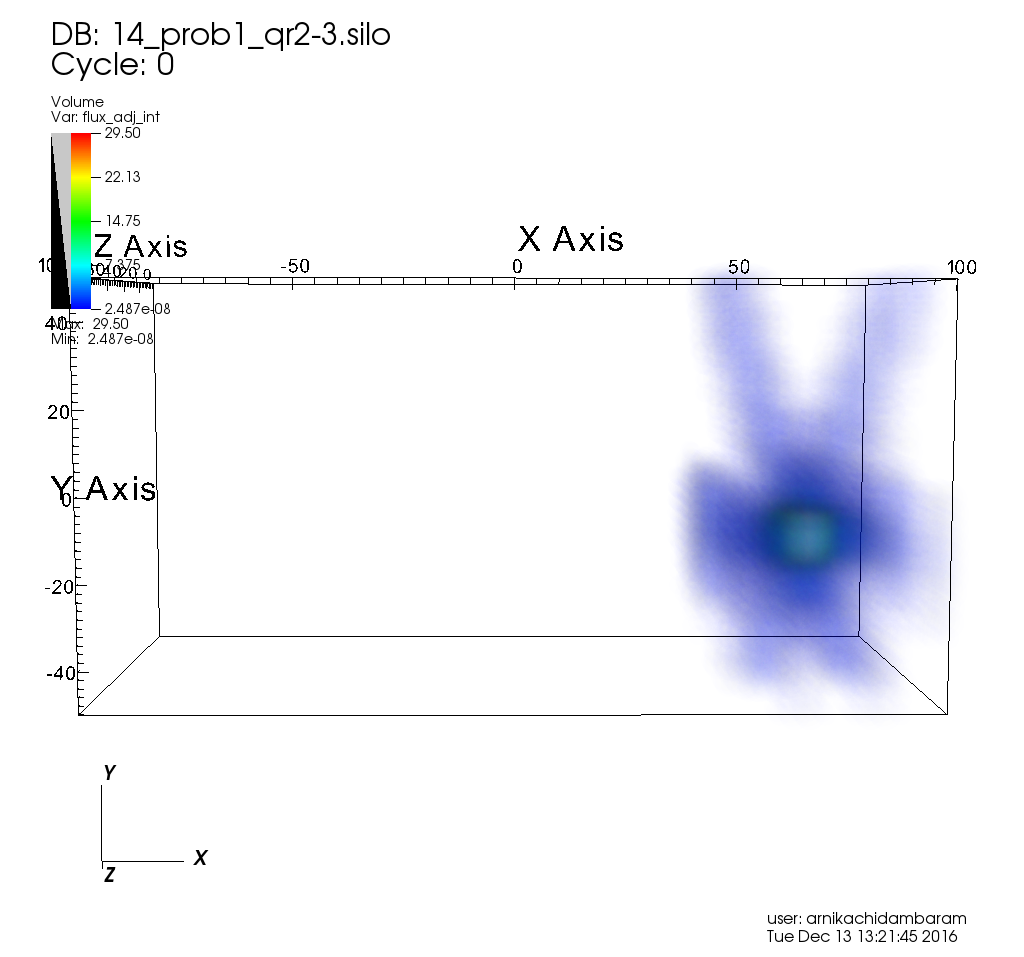
\includegraphics[width = 0.9\textwidth]{visit/visit-prob_1-02.png}
\caption{Problem one geometry with a quadrature number of 2}
\label{visit:prob_1-02}
\end{subfigure}
\hfill
\begin{subfigure}{0.49\textwidth}
\centering
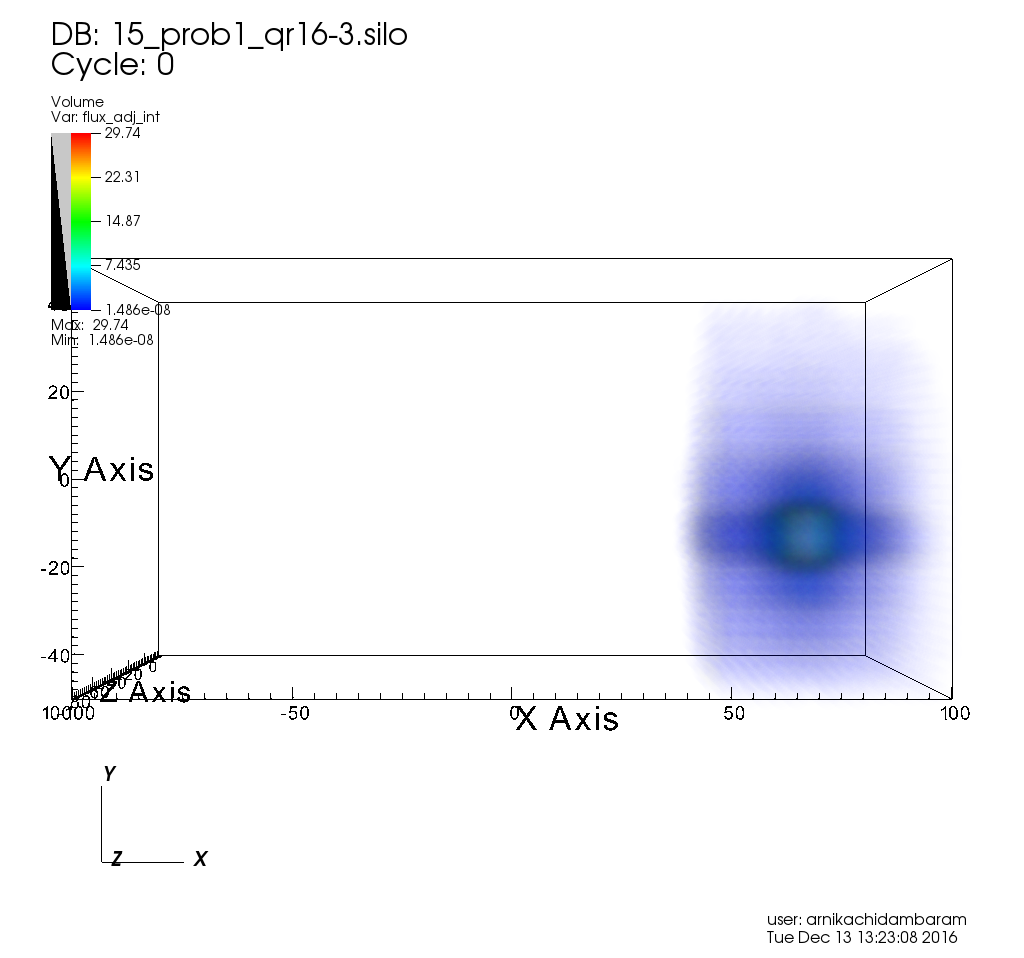
\includegraphics[width = 0.9\textwidth]{visit/visit-prob_1-16.png}
\caption{Problem one geometry with a quadrature number of 16}
\label{visit:prob_1-16}
\end{subfigure}
\caption{Problem 1 Geometry}
\label{visit:prob_1}
\end{figure}

% PROBLEM 2
\begin{figure}[!ht]
\centering
\begin{subfigure}{0.49\textwidth}
\centering
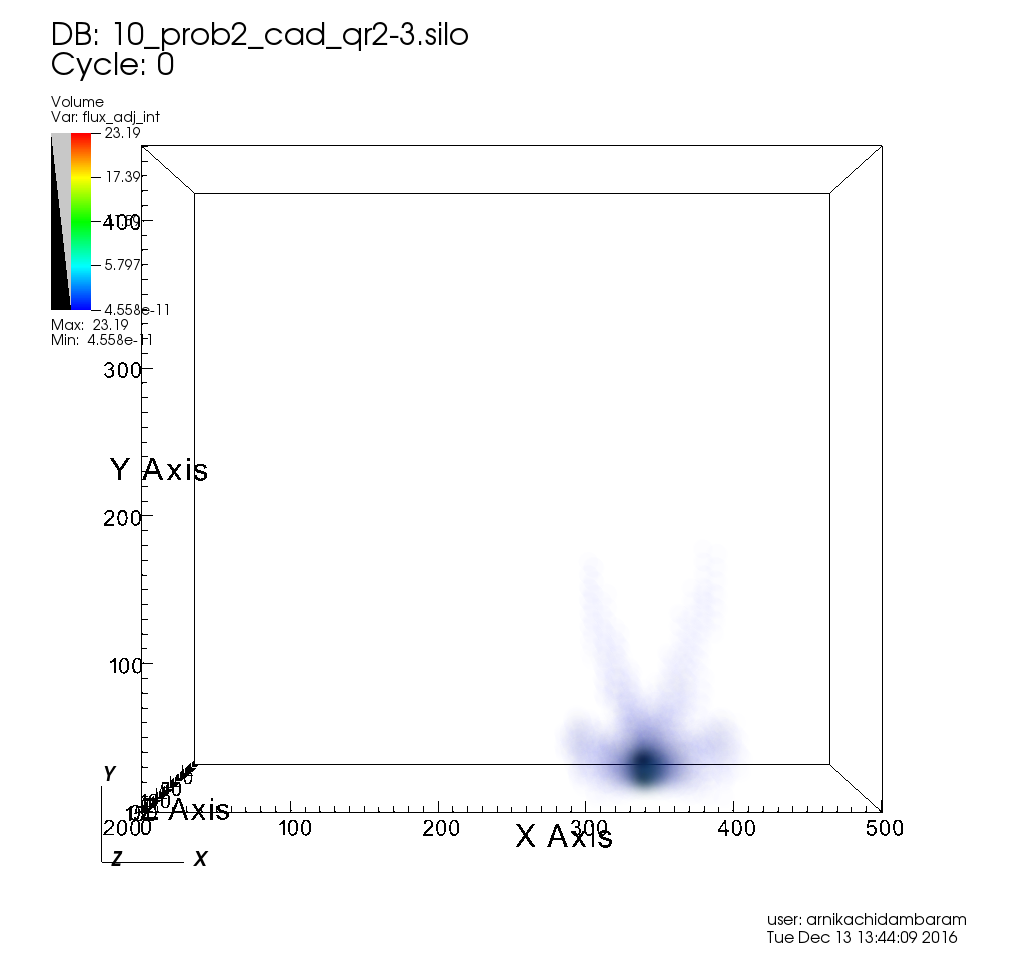
\includegraphics[width = 0.9\textwidth]{visit/visit-prob_2-02}
\caption{Problem two with quadrature number 2}
\label{visit:prob_2-02}
\end{subfigure}
\hfill
\begin{subfigure}{0.49\textwidth}
\centering
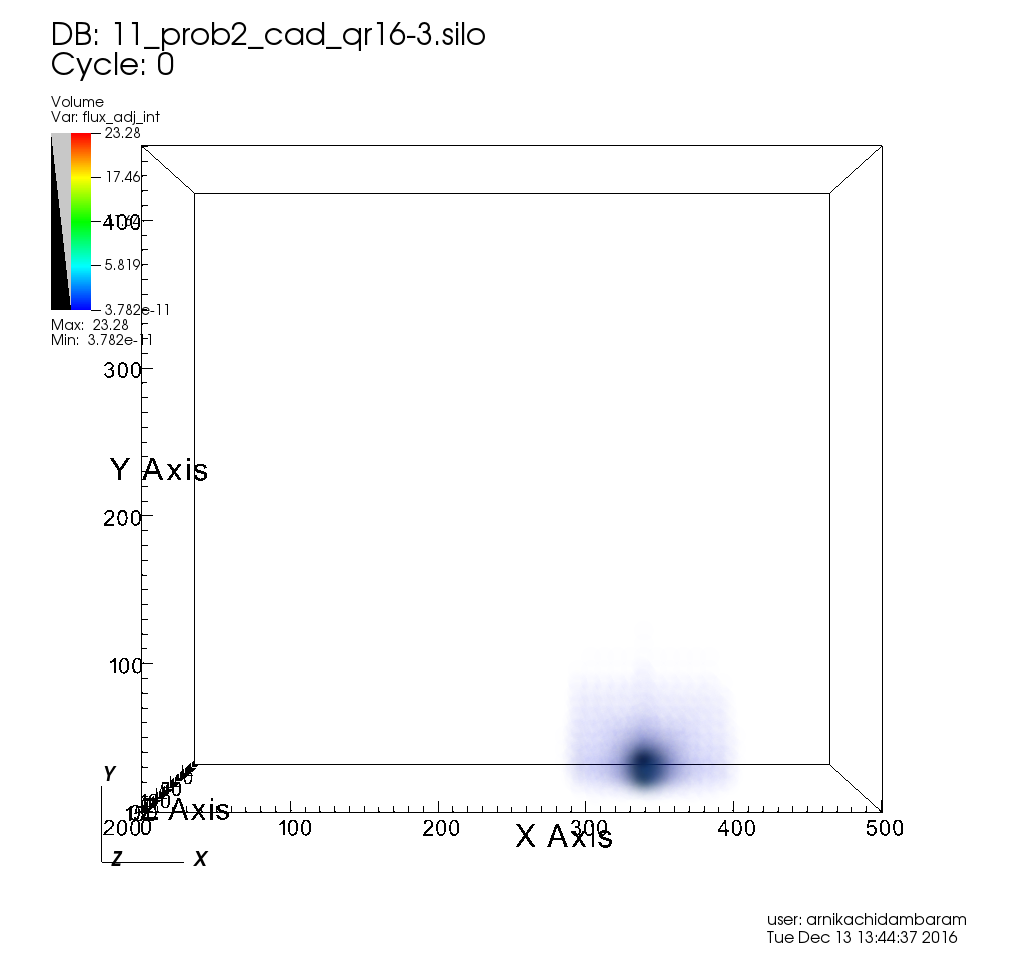
\includegraphics[width = 0.9\textwidth]{visit/visit-prob_2-16}
\caption{Problem two geometry with a quadrature number of 16}
\label{visit:prob_2-16}
\end{subfigure}
\caption{Problem 2 Geometry}
\label{visit:prob_2}
\end{figure}

% PROBLEM 4
\begin{figure}[!ht]
\centering
\begin{subfigure}{0.49\textwidth}
\centering
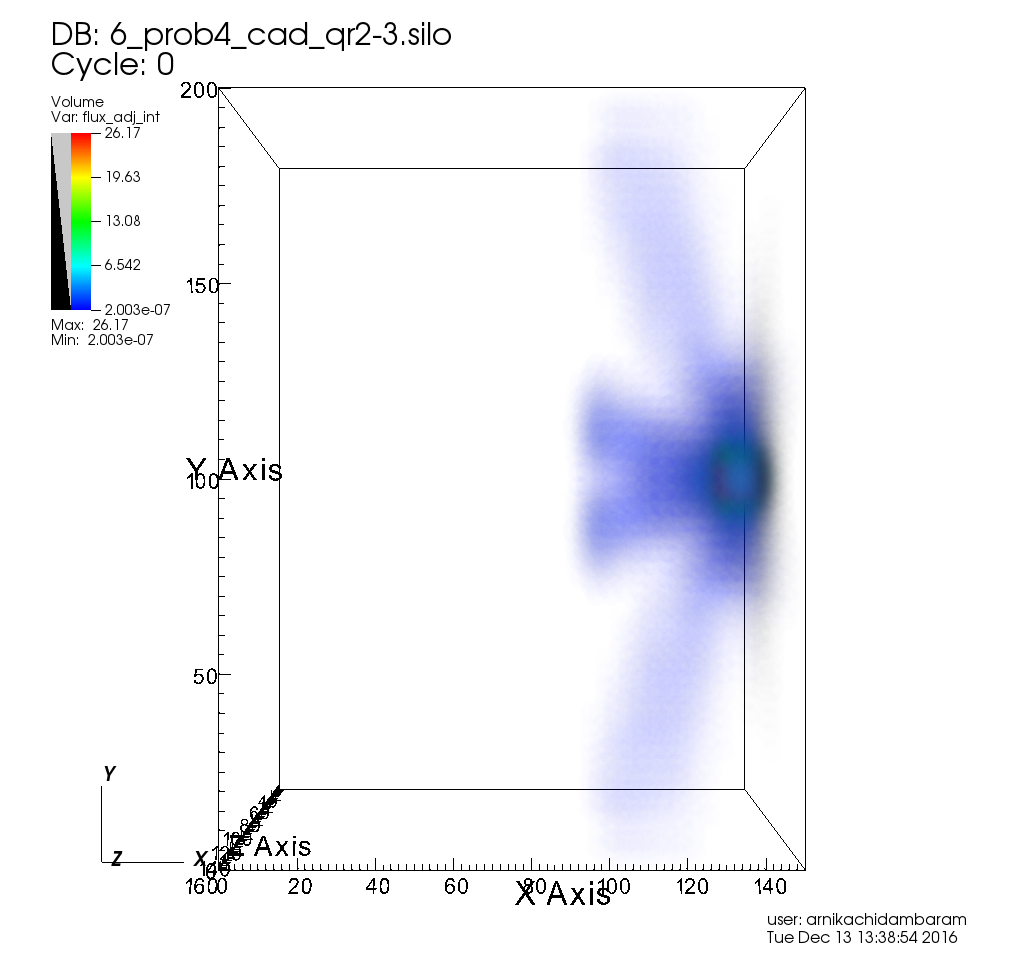
\includegraphics[width = 0.9\textwidth]{visit/visit-prob_4-02}
\caption{Problem four geometry with a quadrature number of 2}
\label{visit:prob_4-02}
\end{subfigure}
\hfill
\begin{subfigure}{0.49\textwidth}
\centering
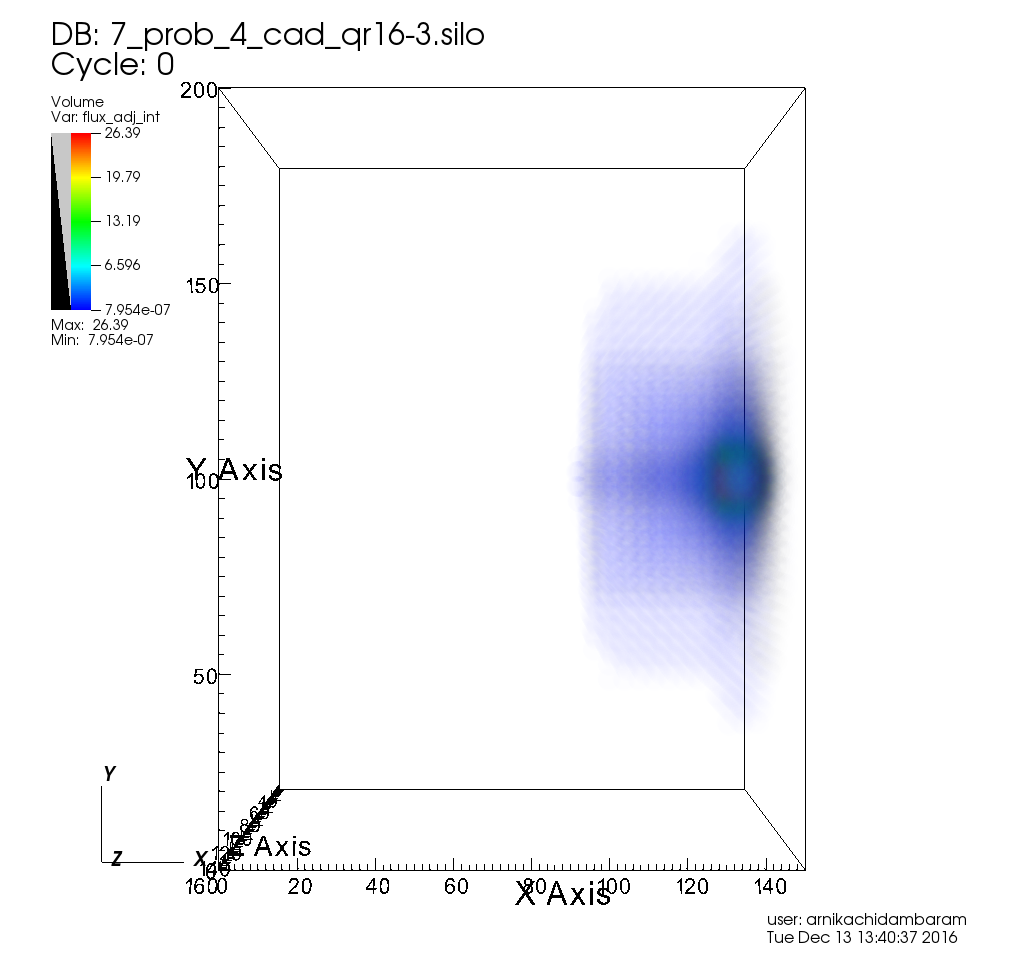
\includegraphics[width = 0.9\textwidth]{visit/visit-prob_4-16}
\caption{Problem four geometry with a quadrature number of 16}
\label{visit:prob_4-16}
\end{subfigure}
\caption{Problem 4 Geometry}
\label{visit:prob_4}
\end{figure}

% MAZE 1
\begin{figure}[!ht]
\centering
\begin{subfigure}{0.49\textwidth}
\centering
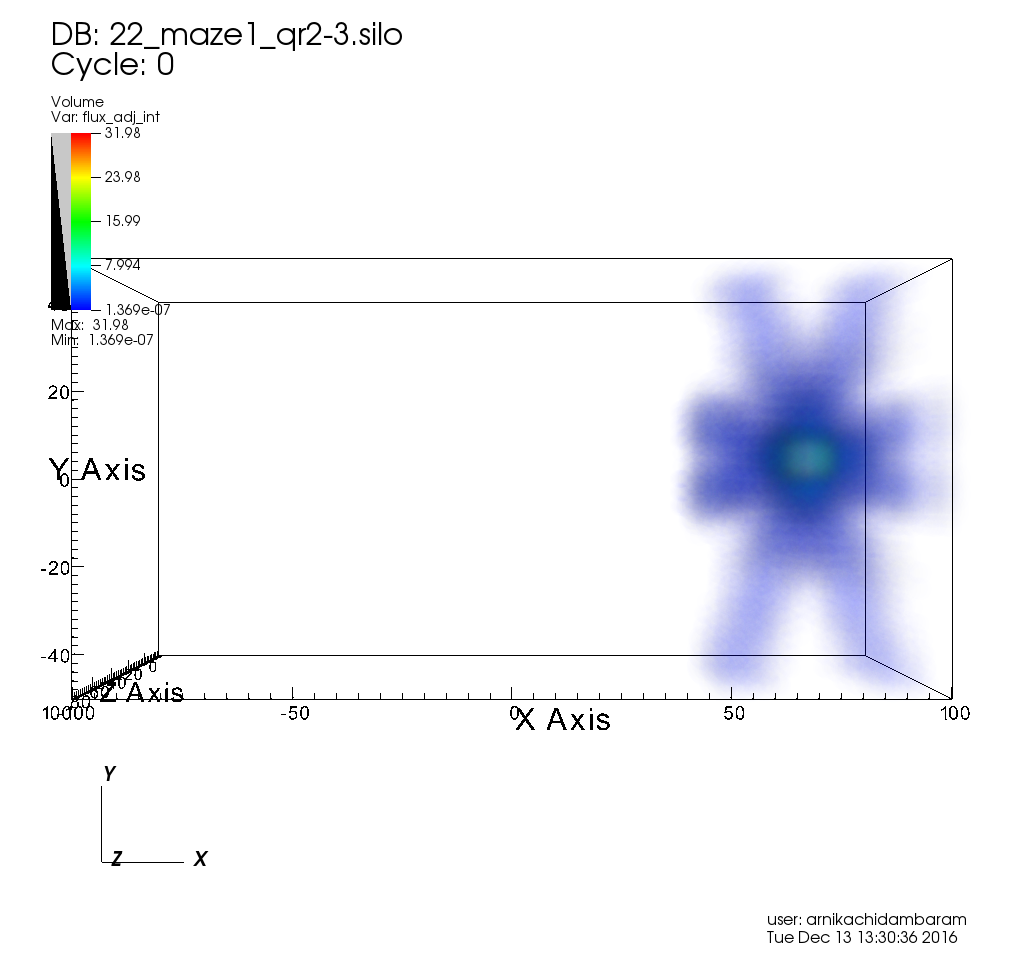
\includegraphics[width = 0.9\textwidth]{visit/visit-maze1-02}
\caption{Maze 1 with quadrature number 2}
\label{visit:maze1-02}
\end{subfigure}
\hfill
\begin{subfigure}{0.49\textwidth}
\centering
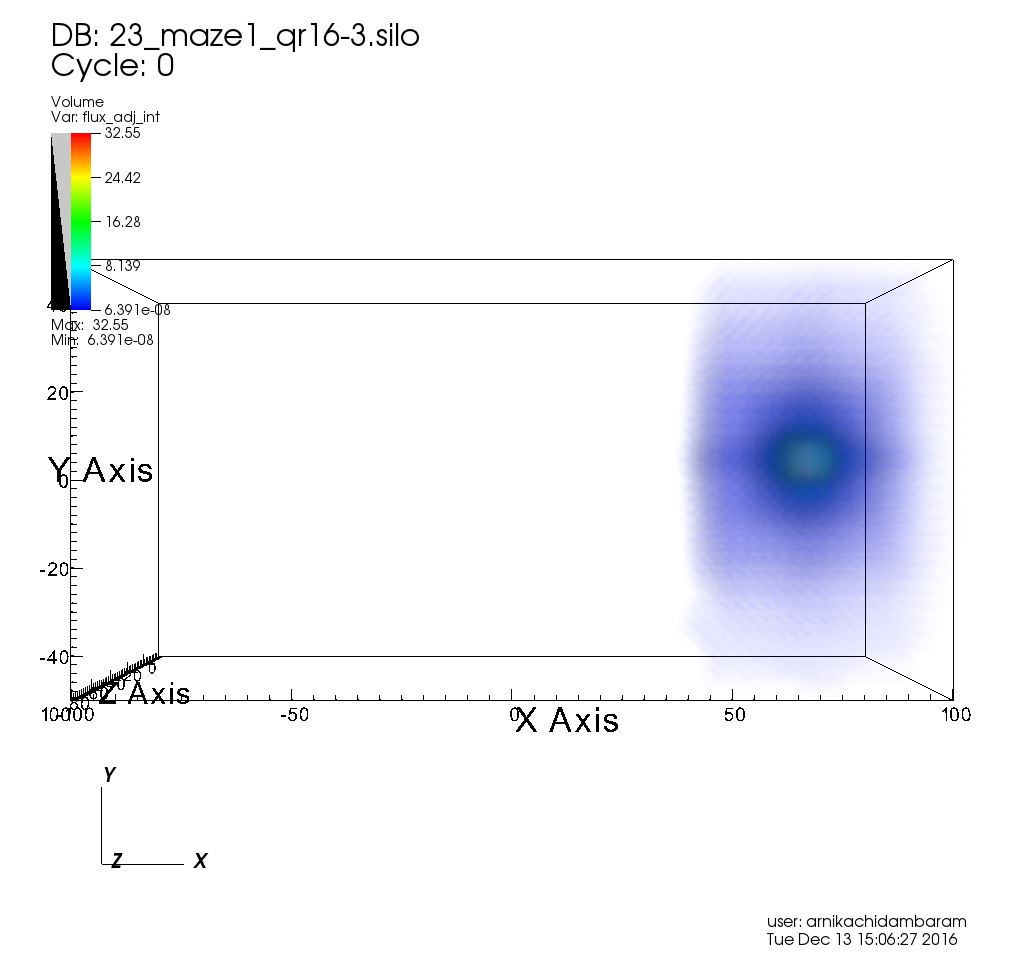
\includegraphics[width = 0.9\textwidth]{visit/visit-maze1-16}
\caption{Maze 1 with quadrature number 16}
\label{visit:maze1-16}
\end{subfigure}
\caption{Maze 1 Geometry}
\label{visit:maze1}
\end{figure}

% MAZE 1
\begin{figure}[!ht]
\centering
\begin{subfigure}{0.49\textwidth}
\centering
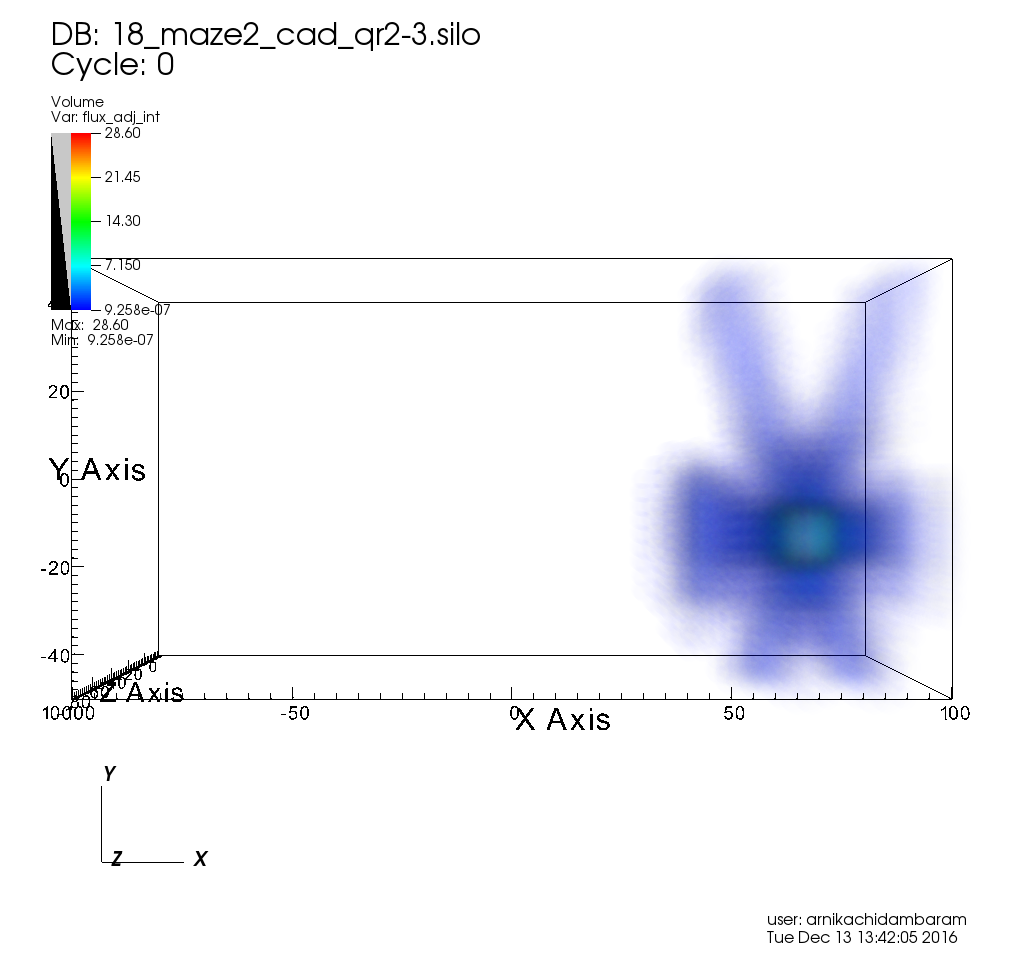
\includegraphics[width = 0.9\textwidth]{visit/visit-maze2-02}
\caption{Maze 2 geometry with quadrature number 2}
\label{visit:maze2-02}
\end{subfigure}
\hfill
\begin{subfigure}{0.49\textwidth}
\centering
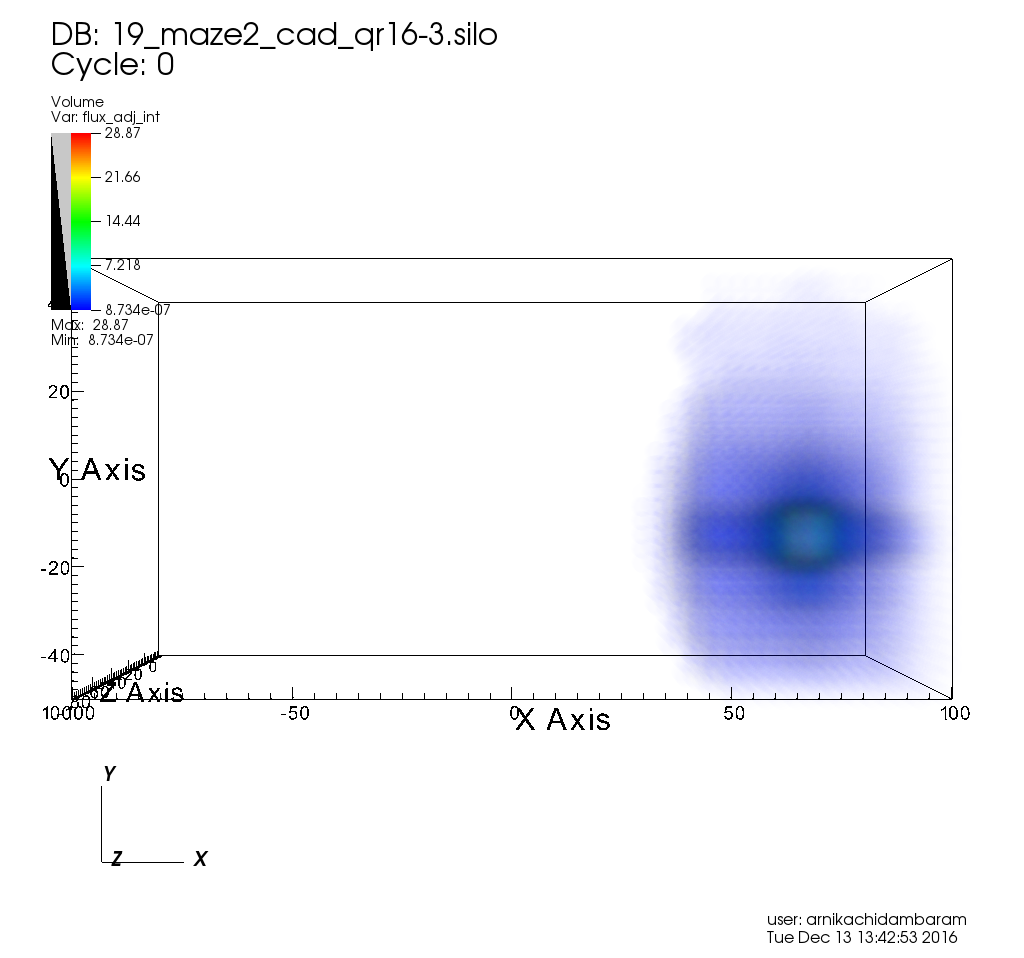
\includegraphics[width = 0.9\textwidth]{visit/visit-maze2-16}
\caption{Maze 2 geometry with quadrature number 16}
\label{visit:maze2-16}
\end{subfigure}
\caption{Maze 2 Geometry}
\label{visit:maze2}
\end{figure}

% BEAM
\begin{figure}[!ht]
\centering
\begin{subfigure}{0.49\textwidth}
\centering
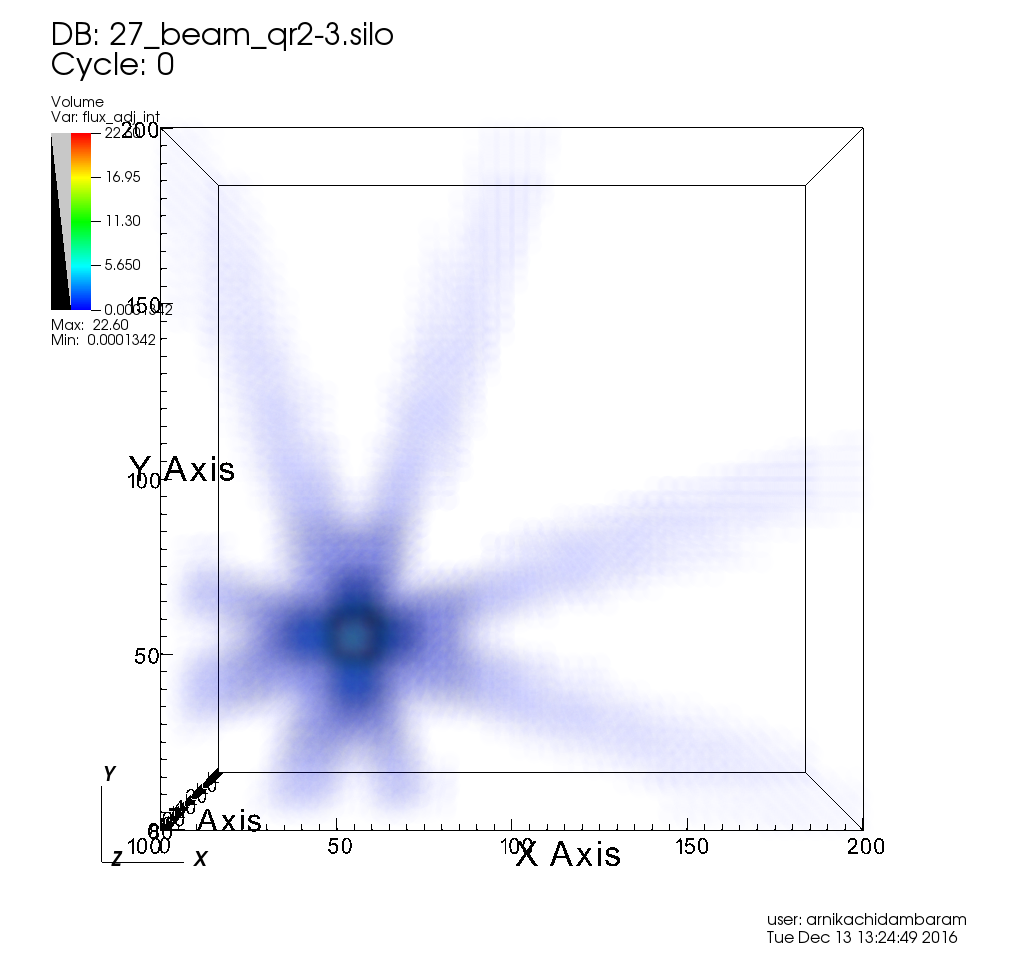
\includegraphics[width = 0.9\textwidth]{visit/visit-beam-02}
\caption{Beam with quadrature number 2}
\label{visit:beam-02}
\end{subfigure}
\hfill
\begin{subfigure}{0.49\textwidth}
\centering
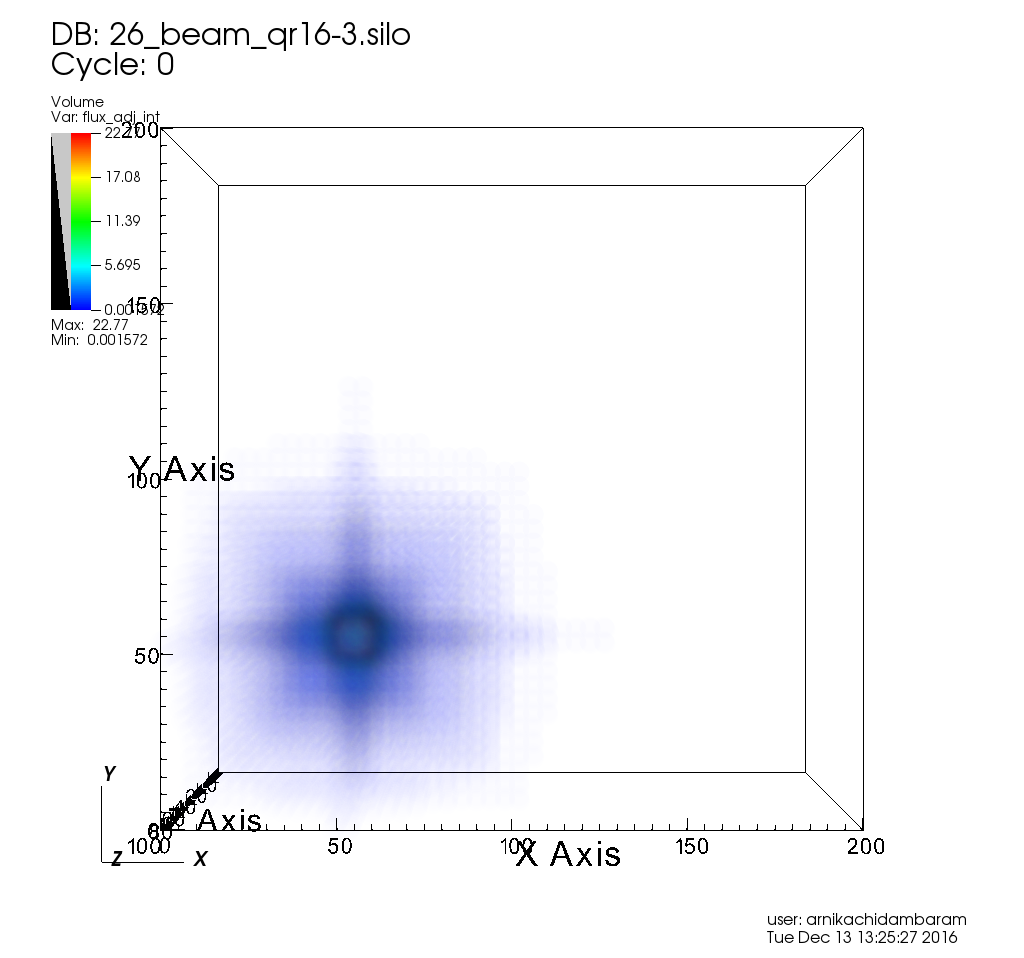
\includegraphics[width = 0.9\textwidth]{visit/visit-beam-16}
\caption{Beam with quadrature number 16}
\label{visit:beam-16}
\end{subfigure}
\caption{Beam Geometry}
\label{visit:beam}
\end{figure}

% THERAPY ROOM
\begin{figure}[!ht]
\centering
\begin{subfigure}{0.49\textwidth}
\centering
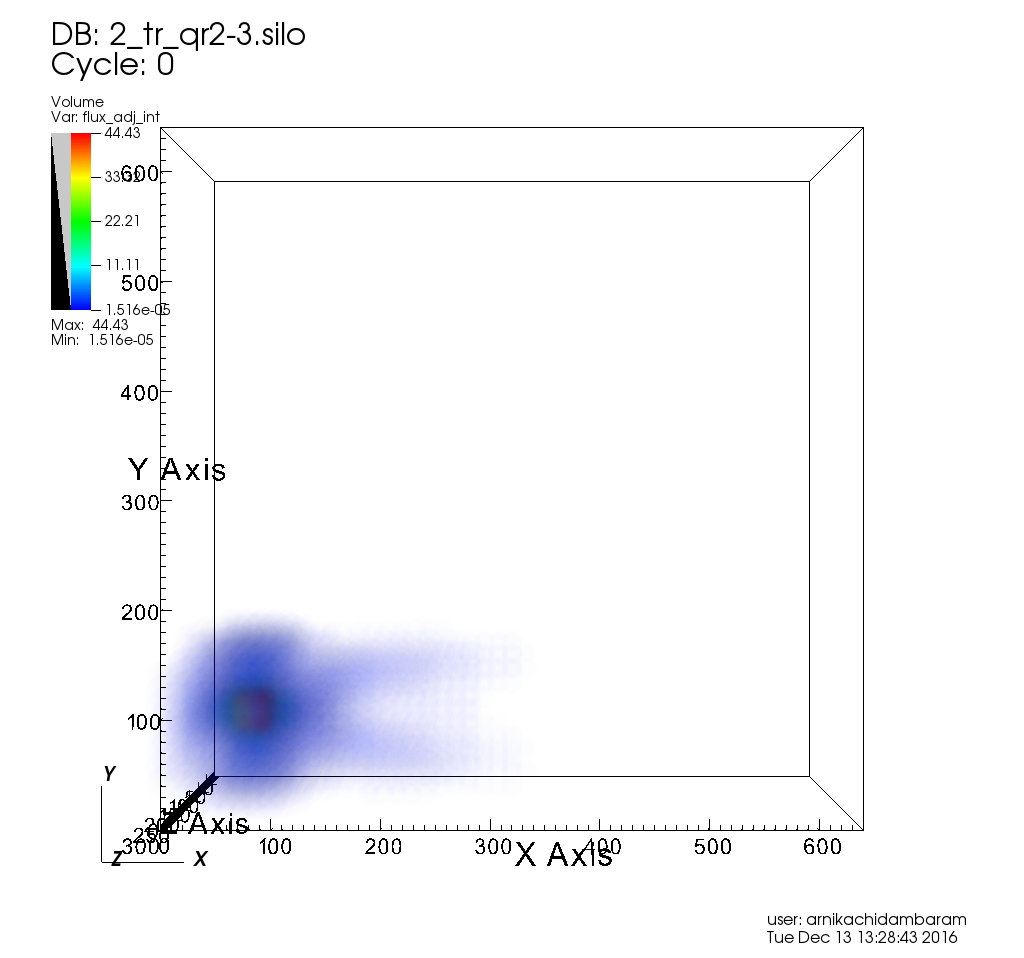
\includegraphics[width = 0.9\textwidth]{visit/visit-therapy-room-02}
\caption{Therapy Room geometry with quadrature number 2}
\label{visit:therapy-room-02}
\end{subfigure}
\hfill
\begin{subfigure}{0.49\textwidth}
\centering
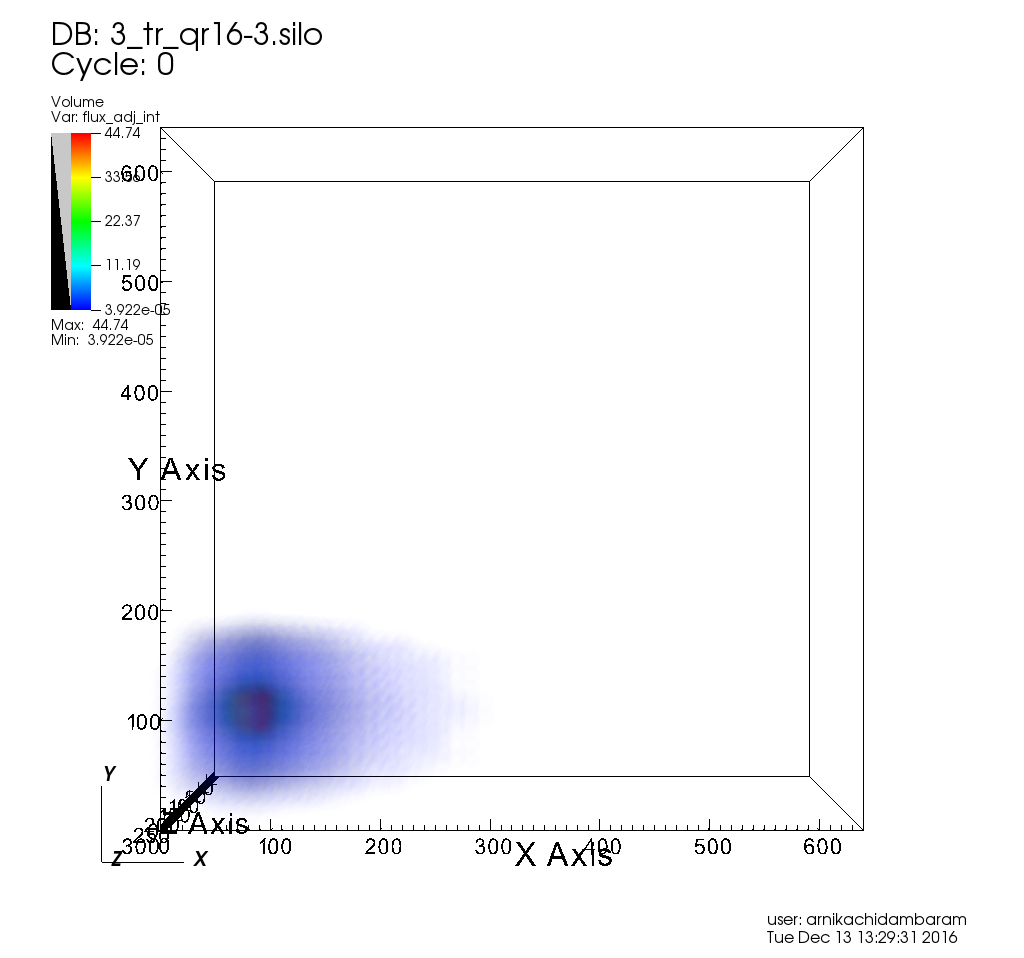
\includegraphics[width = 0.9\textwidth]{visit/visit-therapy-room-16}
\caption{Therapy Room geometry with quadrature number 16}
\label{visit:therapy-room-16}
\end{subfigure}
\caption{Therapy Room Geometry}
\label{visit:therapy-room}
\end{figure}

From the figures, it is apparent that the source ``spreads'' as quadrature number increases.
Ray effects occur because the discrete ordinates method is exact for certain angles but the accuracy at point off those angles is unknown \cite{slaybaugh:discretization}.
In cases with point sources in large spaces, the flux shape distorts. The distorted flux extends out in different directs, resembling the shape of a star, when realistically, it should be spherical in shape.
Increasing the quadrature number spreads the point source across the space and allows it to diffuse, creating a sphere like shape \cite{lewis-and-miller}.
Initially, a volume was defined for each mesh and a source term was assigned to it, for each plot.
However, assigning a source term to each mesh resulted in plots that were either empty or completely identical (and thus unaffected by quadrature number) as seen in \cref{visit:source-term-treatment-room-02,visit:source-term-maze1-02,visit:source-term-maze1-02,visit:source-term-treatment-room-16}

\begin{figure}[!ht]
\begin{subfigure}{0.49\textwidth}
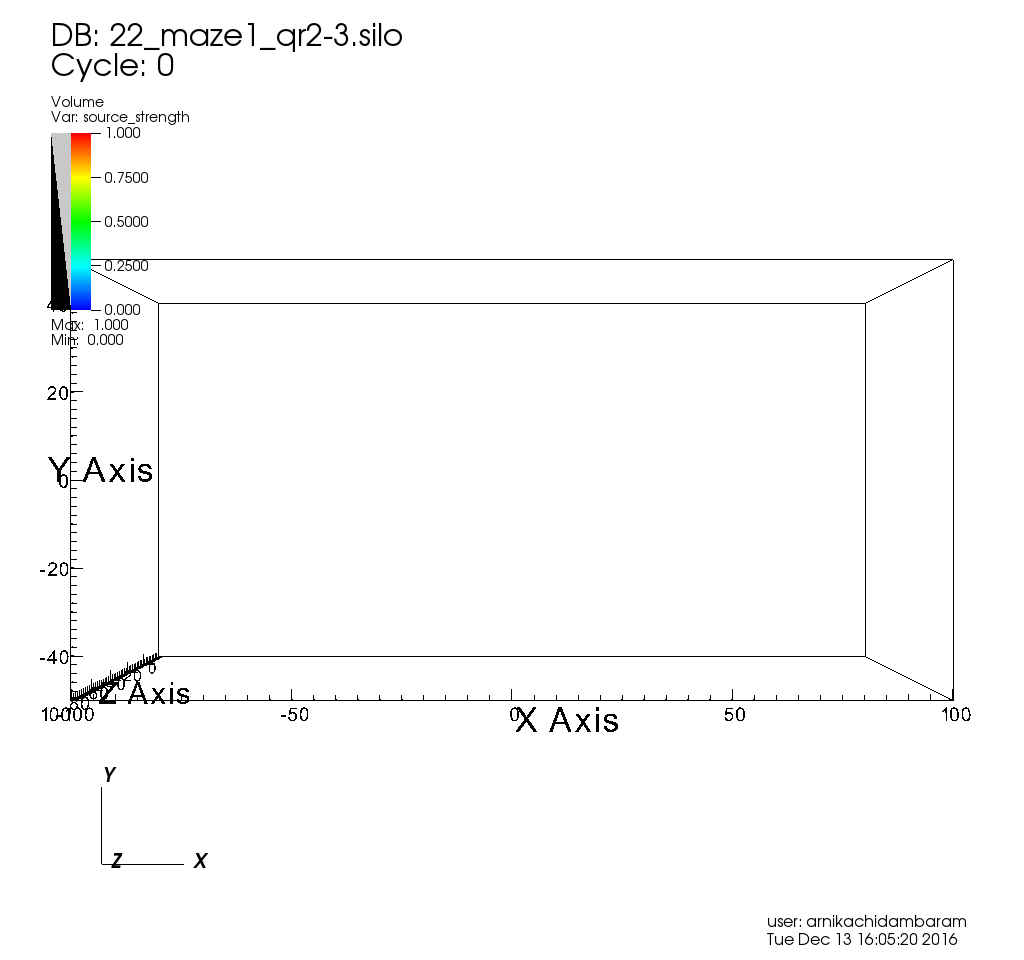
\includegraphics[width = 0.9\textwidth]{visit/source-term-maze1-02}
\caption{Maze 1 geometry with quadrature number 2, plotted with respect to source term}
\label{visit:source-term-maze1-02}
\end{subfigure}
\hfill
\begin{subfigure}{0.49\textwidth}
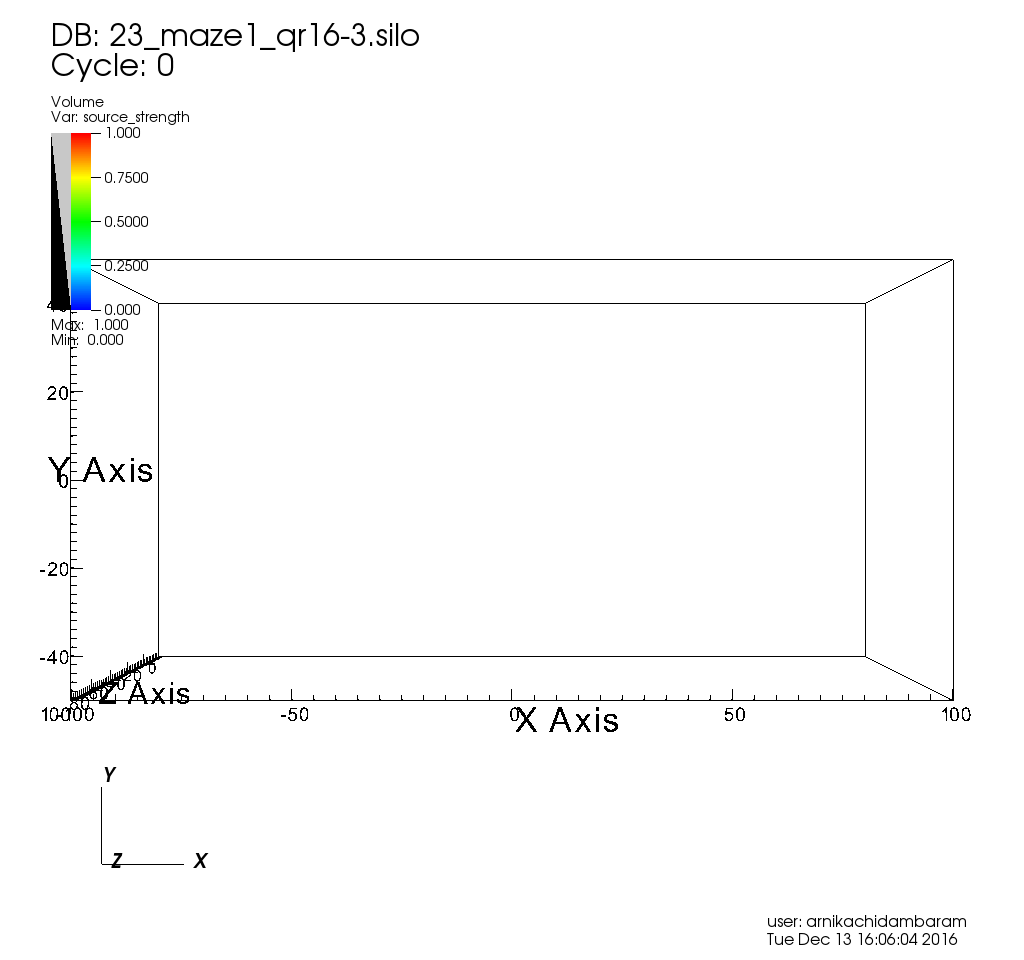
\includegraphics[width = 0.9\textwidth]{visit/source-term-maze1-16}
\caption{Maze 1 geometry with quadrature number 16, plotted with respect to source term}
\label{visit:source-term-maze1-16}
\end{subfigure}

\begin{subfigure}{0.49\textwidth}
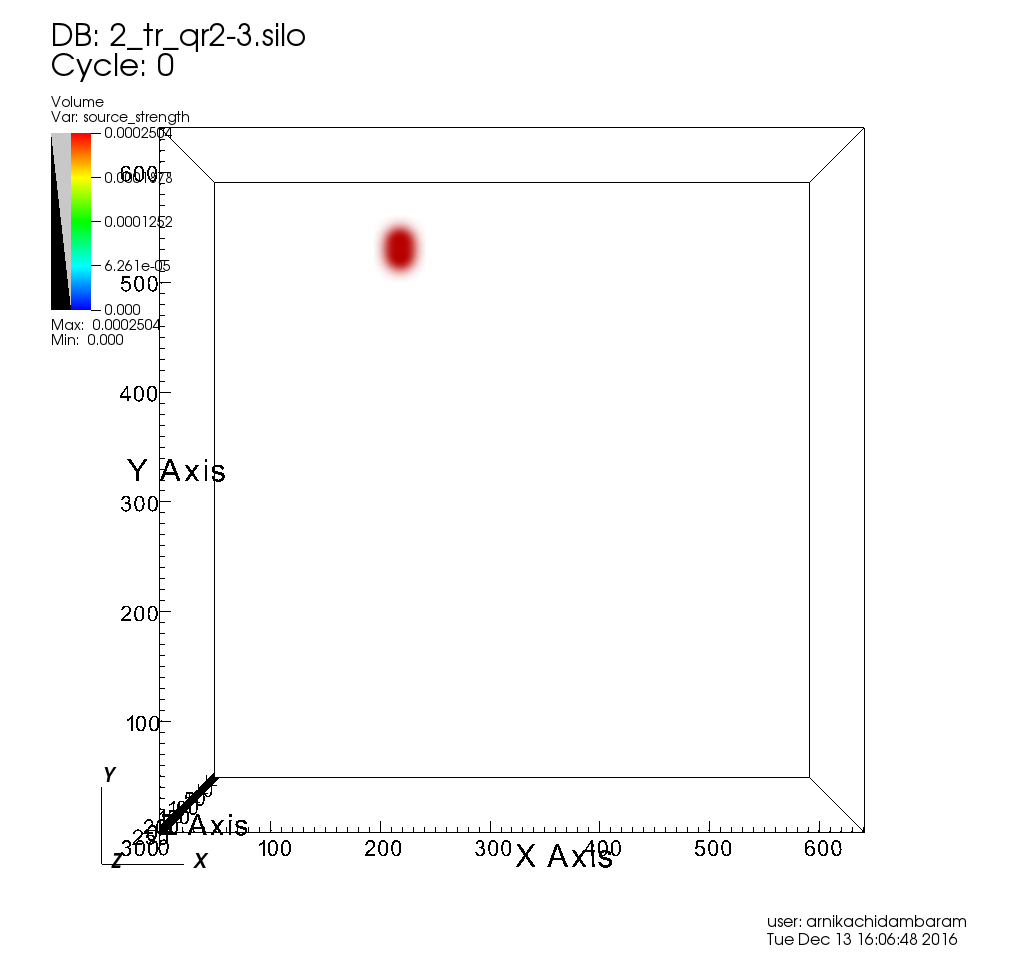
\includegraphics[width = 0.9\textwidth]{visit/source-term-treatment-room-02}
\caption{Therapy Room with quadrature number 2, plotted with respect to source term}
\label{visit:source-term-treatment-room-02}
\end{subfigure}
\hfill
\begin{subfigure}{0.49\textwidth}
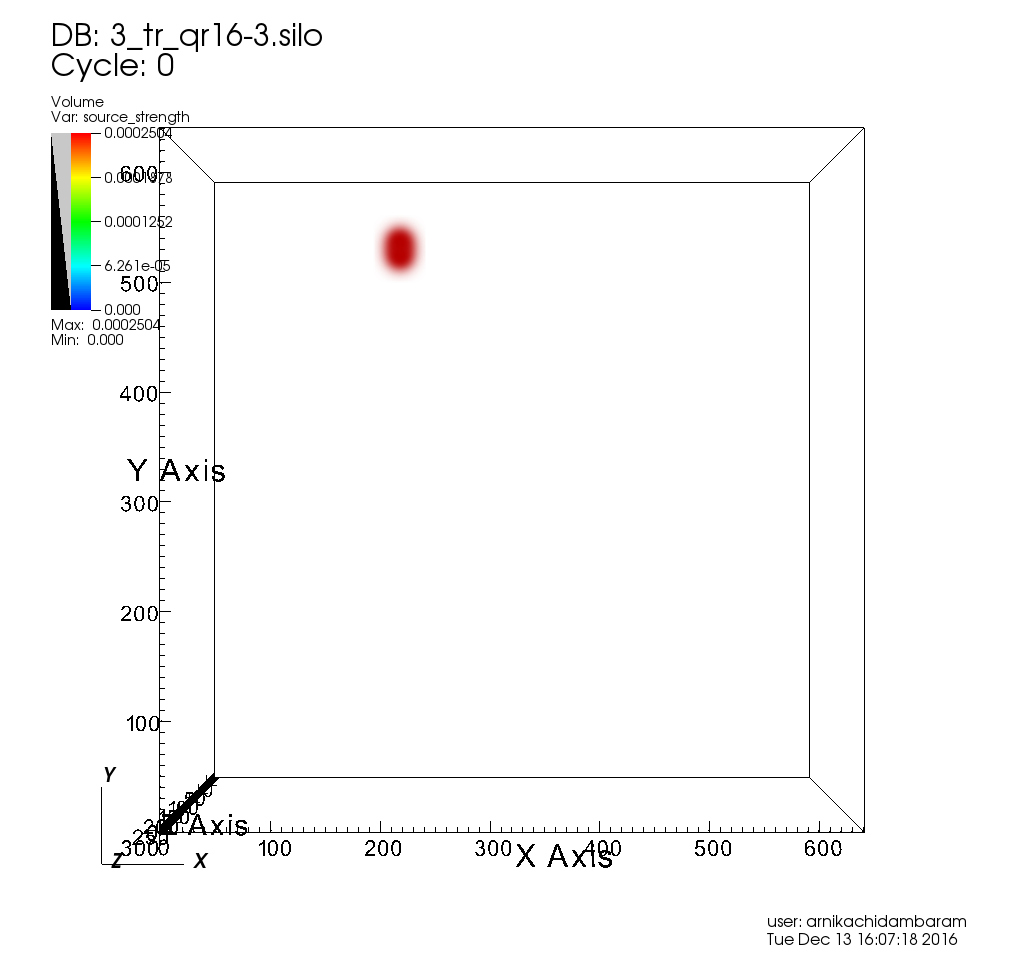
\includegraphics[width = 0.9\textwidth]{visit/source-term-treatment-room-16}
\caption{Therapy Room with quadrature number 16, plotted with respect to source term}
\label{visit:source-term-treatment-room-16}
\end{subfigure}
\end{figure}

After getting help from Madicken, source term was discarded in favor of integral flux and this gave a better trend in terms of quadrature number.
The major drawback of plotting in VisIt was the amount of time it took to understand VisIt, and the amount of time it took to actually generate silo files for each case.
In the future, now that there is a better understanding of Visit, it might be useful to plot more silo files (instead of just the ones that increase quadrature order) so that more trends can be recognized.

\newpage

%%%%%%%%%%%%%%%%%%%%%%%%%%%%%%%%%%%%%%%%%%%%%%%%%%%%%%%%%%%%%%%%%%%%%%%
%  TEST PROBLEMS AND RESULTS -- Describe any testing we did to
%      demonstrate our code is correct and present any results from
%      test problems.
%%%%%%%%%%%%%%%%%%%%%%%%%%%%%%%%%%%%%%%%%%%%%%%%%%%%%%%%%%%%%%%%%%%%%%%
\section{Test Projects and Results}
\label{sec:test}

We ran the simulations for the beam, maze1, maze2, prob$\_$1, prob$\_$2, prob$\_$4, each simulation, we looked at the maximum relative error, simulation run time, and both MCNP and adjusted figure of merit, where the adjusted FOM includes the Denovo run time as well as the MCNP run time.
For CADIS, it was possible to plot both the tally output results and relative errors as functions of energy bin.
For both CADIS and FW-CADIS, we plotted histograms of the distribution of the relative errors.
Examples of these four plots are shown in \cref{maze1-cad,maze1-fwc}.

\begin{figure}[!ht]
\centering
\begin{subfigure}{0.49\textwidth}
\centering
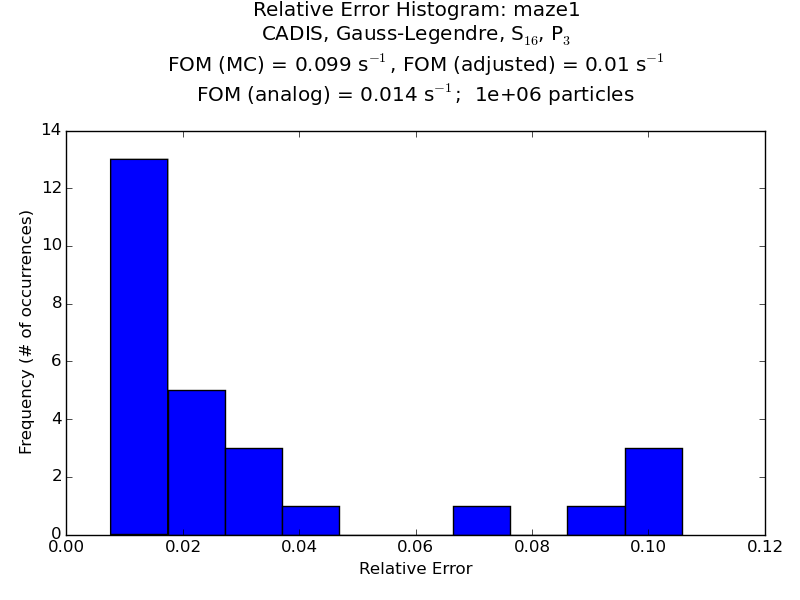
\includegraphics[width = \textwidth]{hist-cad-maze1-GL16.png}
\caption{Histogram of Relative Error for CADIS}
\label{maze1-cad}
\end{subfigure}
\hfill
\begin{subfigure}{0.49\textwidth}
\centering
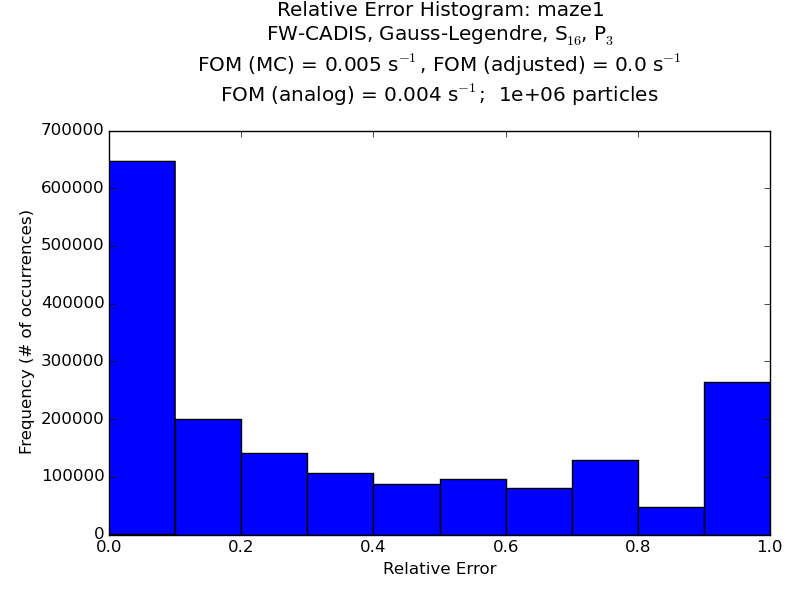
\includegraphics[width = \textwidth]{hist-fwc-maze1-GL16.png}
\caption{Histogram of Relative Error for FW-CADIS}
\label{maze1-fwc}
\end{subfigure}
\caption{Maze 1 Geometry}
\label{maze1}
\end{figure}

\begin{figure}[!ht]
\centering
\begin{subfigure}{0.49\textwidth}
\centering
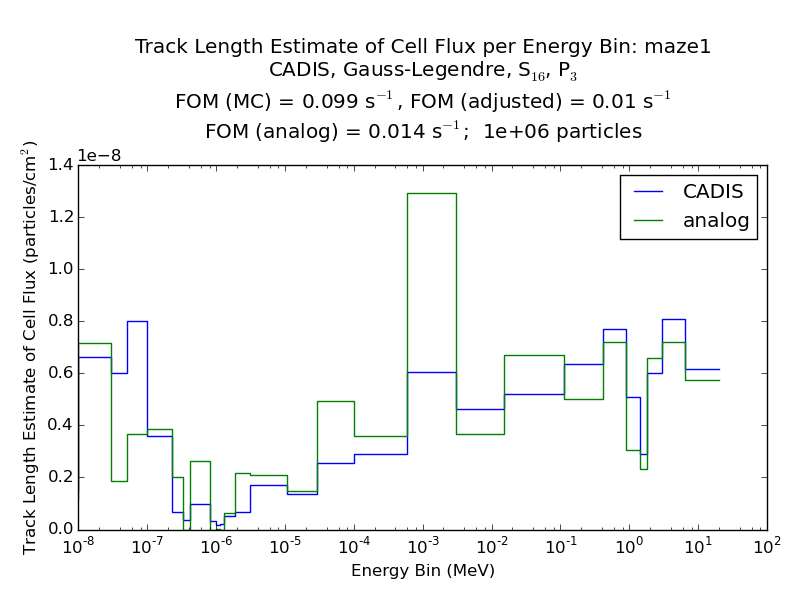
\includegraphics[width = \textwidth]{tally-maze1-GL16.png}
\caption{Relative error vs. of energy bin}
\label{maze1-cad}
\end{subfigure}
\hfill
\begin{subfigure}{0.49\textwidth}
\centering
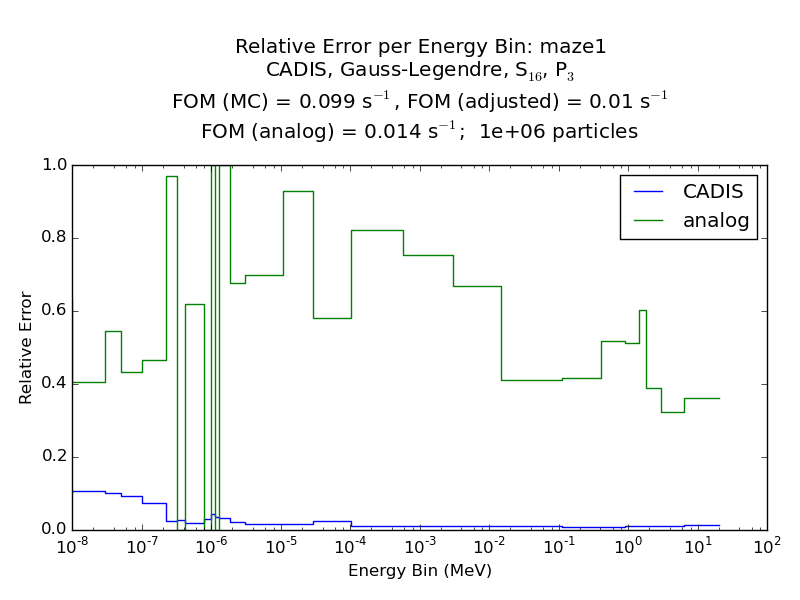
\includegraphics[width = \textwidth]{sigma-maze1-GL16.png}
\caption{Relative error vs. of energy bin}
\label{maze1-fwc}
\end{subfigure}
\caption{Maze 1 Geometry for CADIS}
\label{maze1}
\end{figure}

% %%%%%%%%%%%%%%%%%%%%%%%%%%%%%%%%%%%%%%%%%%%%%%%%%%%%%%%%%%%%%%%%%%%%%%%
% %  PLANS FOR COMPLETION -- What still needs to be done to complete our
% %      project and how will we do it?
% %%%%%%%%%%%%%%%%%%%%%%%%%%%%%%%%%%%%%%%%%%%%%%%%%%%%%%%%%%%%%%%%%%%%%%%
% \newpage
% \section{Plans for Completion}
% \label{sec:plans}
% %\sectionauthor{Caroline, Mitch}

% After careful study of the mathematical background required for our project, the remainder of the project can be divided into two major components: automation and optimization.
% The updated timeline divided by subject area with consideration of time required to write the final report and presentation is as follows:

% \vspace{2ex}

% \singlespacing
% %%%%%%%%%%%%%%%%%%%%%%%%%%%%%%%%%%%%%%%%%%%%%%%%
% \noindent\emph{Automation}

% \begin{center}
% \begin{tabularx}{0.95\textwidth}{rX}
% Tu 11/22    &   Read and store Denovo run times
%                 \newline
%                 Read and store MCNP run times and results   \\
% F~ 11/25    &   Write ADVANTG files.
%                 \newline
%                 Inspect Silo file and visualize using VisIt
%                 \newline
%                 Run MCNP input file in MCNP command window  \\
% Su 11/27    &   Complete automation.
% \end{tabularx}
% \end{center}

% %%%%%%%%%%%%%%%%%%%%%%%%%%%%%%%%%%%%%%%%%%%%%%%%
% \newpage
% \noindent\emph{Characterization Tests}

% \begin{center}
% \begin{tabularx}{0.95\textwidth}{rX}
% F~ 12/02    &   Finish running Maze1, Maze2 and Prob-1 test cases:
% \\
% Su 12/04    &   Finish running Prob-2, Prob-4 and Beam test cases:
% \\
% Tu 12/06    &   Finish running Reactor, WS and Therapy Room test cases:
% \\
% Th  12/08   &
% For each test case, study uncertainty in results and Denovo and MCNP run times for the input parameters listed in \cref{tab:parameter-tests}.
% Plot relationships to analyze.
% \end{tabularx}
% \end{center}

% %%%%%%%%%%%%%%%%%%%%%%%%%%%%%%%%%%%%%%%%%%%%%%%%
% \noindent\emph{Reports and Presentations}

% \begin{center}
% \begin{tabularx}{0.95\textwidth}{rX}
% Sa 12/10    &
% Complete preliminary drafts of the report and presentation.
% \\
% M~ 12/12    &
% Complete final drafts of the report and presentation
% \\
% W~ 12/14    &
% Submit final report and present
% \end{tabularx}
% \end{center}
% %%%%%%%%%%%%%%%%%%%%%%%%%%%%%%%%%%%%%%%%%%%%%%%%
% \onehalfspacing

%%%%%%%%%%%%%%%%%%%%%%%%%%%%%%%%%%%%%%%%%%%%%%%%%%%%%%%%%%%%%%%%%%%%%%%
%  SUMMARY -- What did we do and why does it matter?
%%%%%%%%%%%%%%%%%%%%%%%%%%%%%%%%%%%%%%%%%%%%%%%%%%%%%%%%%%%%%%%%%%%%%%%
\section{Summary}

Throughout the course of this project, we performed CADIS and FW-CADIS runs on seven geometries, each with varied parameters. 
We found that test cases for both CADIS and FW-CADIS runs had 

\label{sec:sum}

\printbibliography

\appendix
\section{Code Organization}
\label{app:code-org}

Group files were shared on Savio in the \texttt{/global/scratch/co$\_$nuclear/NE255project/} directory. Consistent and thoughtful file organization was extremely important to the automation process.

\begin{figure}[!ht]
\small
\dirtree{%
.1 /.
.2 cadis.
	.3 beam.
		.4	beam$\_$glproductSN-PN.
		.4	beam$\_$levelsymSN-PN.
		.4	beam$\_$qrSN-PN.
			.5 adj$\_$solution.
				.6 out.
			.5 output.
				.6 inp \\ wwinp \\ beam$\_$qr2-3.sh.
	.3 maze1.
	.3 maze2.
	.3 prob$\_$1.
	.3 prob$\_$2.
	.3 prob$\_$4.
	.3 reactor.
	.3 therapy-room.
	.3 WS$\_$problem.
.2 fwcadis.
}
\caption{}
\label{docs:advantg}
\end{figure}

\begin{figure}[!ht]
\small
\dirtree{%
.1 /.
.2 mcnp$\_$run$\_$base.sh \\
    mcnpbashwriter.py \\
    mcnpoutreader.py \\
    navigator.py.
}
\caption{}
\label{docs:mcnp}
\end{figure}

\begin{table}
\centering
\caption{Compare $P_3$ and $P_5$}
\csvreader[head to column names,
    tabular = cSScSSSSSS,
    table head = \toprule
        &&&& {Max.}
        & \multicolumn{2}{c}{Run Time (\si{\second})}
        & \multicolumn{2}{c}{Figure of Merit (\si{\second^{-1}})}
        \\
          Quadrature
        & {$S_N$}
        & {$P_N$}
        & {Method}
        & {Rel. Err.}
        & {Denovo}
        & {MCNP}
        & {MCNP}
        & {Adjusted}
        \\\midrule,
    table foot = \bottomrule,
    , filter=\equal{\SN}{10},]
    {tab/results.csv}
    {}
    {\quadrature & \SN & \PN & \method & \sigma & \timeDenovo & \timeMCNP & \fomMCNP & \fomAdjusted}
\end{table}


\end{document}


% Things Mitch cut but doesn't want to delete yet...

By definition, the response of a detector is given by 

When considering fixed source problems, the adjoint flux FW-CADIS is ``particularly useful'' for problems with a fixed source $q$ \cite{slaybaugh:deterministic-parameter-study}.
For a detector response at $(\vec{r}_0, E_0, \hat{\Omega}_0)$ the TE becomes \cite{slaybaugh:250-notes:10-19},

%%%%%%%%%%%%%%%%%%%%%%%%%%%%%%%%%%%%%%%%%%%%%%%%
\begin{align*}
H \psi
&=
q
=
\delta(\vec{r}      - \vec{r}_0)
\delta(E            - E_0)
\delta(\hat{\Omega} - \hat{\Omega}_0)\;;
% % 
% %
% \left<
% \psi^\dagger, H \psi
% \right>
% =
% \left<
% \psi^\dagger , q
% \right>
\\
%%%%%%%%%%%%%%%%%%%%%%%%%%%%%%%%%%%%%%%%%%%%%%%%
H^\dagger \psi^\dagger
&=
q^\dagger\;.
%
% &
% %
% \left<
% \psi , H^\dagger \psi^\dagger
% \right>
% &=
% \left<
% \psi, q^\dagger
% \right> = R
\end{align*}
%%%%%%%%%%%%%%%%%%%%%%%%%%%%%%%%%%%%%%%%%%%%%%%%
